\documentclass[journal]{style/vgtc} 			          % final (journal style)
%\documentclass[review,journal]{style/vgtc}         % review (journal style)
%\documentclass[widereview]{style/vgtc}             % wide-spaced review
%\documentclass[preprint,journal]{style/vgtc}       % preprint (journal style)
%\documentclass[electronic,journal]{style/vgtc}     % electronic version, journal
%% Uncomment one of the lines above depending on where your paper is
%% in the conference process. ``review'' and ``widereview'' are for review
%% submission, ``preprint'' is for pre-publication, and the final version
%% doesn't use a specific qualifier. Further, ``electronic'' includes
%% hyperreferences for more convenient online viewing.
%% Please use one of the ``review'' options in combination with the
%% assigned online id (see below) ONLY if your paper uses a double blind
%% review process. Some conferences, like IEEE Vis and InfoVis, have NOT
%% in the past.

%% Please note that the use of figures other than the optional teaser is not permitted on the first page
%% of the journal version.  Figures should begin on the second page and be
%% in CMYK or Grey scale format, otherwise, colour shifting may occur
%% during the printing process.  Papers submitted with figures other than the optional teaser on the
%% first page will be refused.

%% These three lines bring in essential packages: ``mathptmx'' for Type 1
%% typefaces, ``graphicx'' for inclusion of EPS figures. and ``times''
%% for proper handling of the times font family.

\usepackage{mathptmx}
\usepackage{graphicx}
\usepackage{times}
% TODO: Self added Packages - need to be removed afterwards
%\usepackage{babel}
\usepackage[normalem]{ulem}
%\usepackage{color}
\usepackage{xcolor}
\newcommand{\rem}[1]{\textcolor{red}{\sout{#1}}}
\newcommand{\add}[1]{\textcolor{blue}{\uline{#1}}}
\newcommand{\com}[1]{\textcolor{orange}{\uline{#1}}}

%% We encourage the use of mathptmx for consistent usage of times font
%% throughout the proceedings. However, if you encounter conflicts
%% with other math-related packages, you may want to disable it.

%% This turns references into clickable hyperlinks.
\usepackage[bookmarks,backref=true,linkcolor=black]{hyperref} %,colorlinks
\hypersetup{
  pdfauthor = {},
  pdftitle = {},
  pdfsubject = {},
  pdfkeywords = {},
  colorlinks=true,
  linkcolor= black,
  citecolor= black,
  pageanchor=true,
  urlcolor = black,
  plainpages = false,
  linktocpage
}

%% If you are submitting a paper to a conference for review with a double
%% blind reviewing process, please replace the value ``0'' below with your
%% OnlineID. Otherwise, you may safely leave it at ``0''.
\onlineid{194}

%% declare the category of your paper, only shown in review mode
\vgtccategory{Research}

%% allow for this line if you want the electronic option to work properly
\vgtcinsertpkg

%% In preprint mode you may define your own headline.
%\preprinttext{To appear in an IEEE VGTC sponsored conference.}

%% Paper title.

\title{Interactive Visual Analysis of Image-Centric Cohort Study Data}

%% This is how authors are specified in the journal style

%% indicate IEEE Member or Student Member in form indicated below
\author{Paul Klemm$^{1}$, Steffen Oeltze-Jafra$^{1}$, Kai Lawonn$^{1}$, Katrin Hegenscheid$^{2}$, Henry V{\"o}lzke$^{2}$, Bernhard Preim$^{1}$}
\authorfooter{
%% insert punctuation at end of each item
\item
 $^1$Otto-von-Guericke University Magdeburg, Germany.
\item
 $^2$Ernst-Moritz-Arndt-University Greifswald, Germany.
}

%other entries to be set up for journal
\shortauthortitle{Klemm \MakeLowercase{\textit{et al.}}: Interactive Visual Analysis of Image-Centric Cohort Study Data}
%\shortauthortitle{Firstauthor \MakeLowercase{\textit{et al.}}: Paper Title}

%% Abstract section.
\abstract{%
%(The problem).
%
%The data are analyzed using a priori defined hypotheses to find statistically significant correlations between features (\emph{associations}).
%
%Modern cohort studies incorporate medical image data.
%
%
%The statistically driven epidemiological workflow only allows to determine \emph{associations} between image-derived metrics, such as distances extracted from landmarks of the segmentation model.
%\\\\
% ----------- OLD ABSTRACT ---------
% Epidemiological population studies impose information about a set of subjects (a \emph{cohort}) to characterize disease-specific risk factors.
% %
% Cohort studies comprise of heterogenous variables (\emph{features}) describing the medical condition as well as demographic and lifestyle factors and more recently, medical image data.
% %(New Solution).
% We propose an Interactive Visual Analysis (\emph{IVA}) approach that enables epidemiologists to examine both image-based as well as non-image data, e.g., sociodemographic features and attributes derived from the image data.
% %
% This is achieved by combining brushing and linking enabled coordinated information visualization views and interactive 3D shape renderings with epidemiological data representations such as pivot tables and key figures as association measures.
% %(Validation).
% The presented concepts are applied by experts to gather and evaluate hypotheses about the aging process of the lumbar spine.
% %
% %(Results).
% It allows a more flexible comparison between image and non-image data.
% %
% %(Implications).
% The new framework enables hypotheses validation and generation by incorporating human pattern recognition as well as data mining methods.
% %
% Using all reliable information from the image segmentation linked to non-image features aims to unveil \emph{associations} by applying an iterative analysis approach.
% ----------- /OLD ABSTRACT ---------
\add{%Large-scale longitudinal epidemiological studies investigate groups of people with common characteristics or experiences (a cohort) to characterize health and identify disease-specific risk factors.
%
%Cohort study data comprise thousands of individuals and hundreds of heterogenuous variables (\emph{features}), describing the medical condition as well as demographic and lifestyle factors, and more recently, medical image data.
Epidemiological population studies impose information about a set of subjects (a \emph{cohort}) to characterize disease-specific risk factors.
%
Cohort studies comprise of heterogenous variables (\emph{features}) describing the medical condition as well as demographic and lifestyle factors and more recently, medical image data.
%
%In the standard epidemiological workflow, a hypothesis is given and validated by analyzing a subset of possibly relevant variables over manually defined subgroups of the cohort, e.g., based on age or body weight.
%
%A potential impact of the neglected variables remains unnoticed, data-driven group definition is not supported, and capabilities for integrating the image data into the analysis are missing.\\
%
We propose an Interactive Visual Analysis (\emph{IVA}) approach that enables epidemiologists to rapidly investigate the entire data pool for \emph{hypothesis validation} and \emph{generation}.
%
We incorporate image data, which involves shape-based object detection and the derivation of attributes describing the object shape.
%
The concurrent investigation of image-based and non-image data is realized in a web-based multiple coordinated view system, comprising standard views from information visualization and epidemiological data representations such as pivot tables.
%
%To account for the numerous categorical variables, a mosaic plot is integrated.
%
The views are equipped with brushing facilities and augmented by 3D shape renderings of the segmented objects, e.g., each bar in a histogram is overlaid with a mean shape of the associated subgroup of the cohort.
%
We integrate an \emph{overview visualization}, clustering of features and object shape for data-driven subgroup definition and statistical key figures for measuring the association between variables.
%
We demonstrate the \emph{IVA} approach by validating and generating hypotheses related to lower back pain as part of a qualitative evaluation.}%and the aging process of the lumbar spine.}
} % end of abstract

%% Keywords that describe your work. Will show as 'Index Terms' in journal
%% please capitalize first letter and insert punctuation after last keyword
\keywords{Interactive Visual Analysis, Epidemiology, Spine}

%% ACM Computing Classification System (CCS). 
%% See <http://www.acm.org/class/1998/> for details.
%% The ``\CCScat'' command takes four arguments.

\CCScatlist{ % not used in journal version
 \CCScat{K.6.1}{Management of Computing and Information Systems}%
{Project and People Management}{Life Cycle};
 \CCScat{K.7.m}{The Computing Profession}{Miscellaneous}{Ethics}
}

%% Uncomment below to include a teaser figure.
  % \teaser{
  % \centering
  % \includegraphics[width=16cm]{CypressView}
  % \caption{In the Clouds: Vancouver from Cypress Mountain.}
  % }

%% Uncomment below to disable the manuscript note
%\renewcommand{\manuscriptnotetxt}{}

%% Copyright space is enabled by default as required by guidelines.
%% It is disabled by the 'review' option or via the following command:
% \nocopyrightspace

%%%%%%%%%%%%%%%%%%%%%%%%%%%%%%%%%%%%%%%%%%%%%%%%%%%%%%%%%%%%%%%%
%%%%%%%%%%%%%%%%%%%%%% START OF THE PAPER %%%%%%%%%%%%%%%%%%%%%%
%%%%%%%%%%%%%%%%%%%%%%%%%%%%%%%%%%%%%%%%%%%%%%%%%%%%%%%%%%%%%%%%%

\begin{document}

%% The ``\maketitle'' command must be the first command after the
%% ``begin{document}'' command. It prepares and prints the title block.

%% the only exception to this rule is the \firstsection command
\firstsection{Introduction}

\maketitle
%% \section{Introduction} %for journal use above \firstsection{..} instead
Epidemiology aims at characterizing health and disease by determining risk factors.
%
Clinical problems, such as the selection of diagnostic tools and efficient treatment, are tackled using results of epidemiological research.
%
Also, the introduction of preventive measures in medicine and beyond is based on epidemiological research, where, for example, subgroups with increased risk are identified \cite{Fletcher2012}.
%
Observations made by clinicians in the daily routine are translated into hypotheses for epidemiological research.
%
These are used to determine environmental and lifestyle factors as well as medical examination results that may influence a disease.
%
Potentially useful data variables (\emph{features}) are gathered using structured interviews and clinical examinations.
%
Methods like regression analysis are employed to check the attribute list for statistical soundness.
%
\\\\
Longitudinal population-based studies, such as the Study of Health in Pomerania (SHIP) \cite{Volzke2011}, gather as much information as possible about a defined sample of people (a \emph{cohort}).
%
The cohort consists of several thousands of people who are randomly selected to avoid any bias.
%
The subjects are selected without focus on a certain disease.
%
A large size of the cohort is therefore essential to investigate differences between healthy and diseased people.
%
% The sample is drawn randomized to avoid selection \cite{Fletcher2012}.
% %
% When for example one investigates risk factors for prostate cancer in male subjects, the outcome is strongly dependent on the age.
% %
% Therefore results need to be age-adjusted to be comparable.
% %
% Confounding variables, are often not obvious at all and characterizing them is already an epidemiological result.
%
Cohort studies often include medical image data.
% .
Segmentation of these data enables an anatomical structure analysis and an analysis of possible correlations with other features.
%
Semi-automatic techniques are more promising but also challenging, since the employed modalities, such as magnetic resonance imaging (MRI) and ultrasound, are subject to inhomogeneity and noise.
%
Analyzing spatial data with respect to other epidemiological factors requires techniques that reach beyond standard statistical methods.

Compiling a list of features for tests of statistical resilience based on experience-driven hypotheses leaves out other features in the data which potentially interact with a disease.
%
This also applies to the chosen landmarks used to quantify medical image data information.
%
The standard workflow lacks methods, which identify correlations that the epidemiologists did not consider.
%
Also, only a small subset of variables can be concurrently analyzed. %depending on the statistical measure.
\\\\
We propose an Interactive Visual Analysis (\emph{IVA}) approach \cite{Thomas2005} for the combined analysis of image and non-image data.
%
Visual queries and direct feedback of Visual Analytics systems allow for a fast exploration of the data space incorporating many different variables.
%
Intended as an extension to the well-established epidemiological tools it provides a way to rapidly validate hypotheses and to trigger \emph{hypothesis generation} using data mining methods, such as clustering.
%
\emph{Hypothesis generation} gains importance since the number of epidemiological features increases and the focus shifts towards more complex relations involving more than two features. Our contributions are:
\begin{itemize}
	\item an \add{IVA} workflow for cohort study data to allow both, hypothesis-driven analysis and hypothesis generation--based on a characterization of the standard epidemiological workflow,
	\item visualization techniques, which incorporate both information visualization and 3D rendering of organ shapes as well as combining them with epidemiological graphics and key figures,
	\item highlighting subject groups and feature associations using shape-based clustering and statistical contingency measures.
	%\item highlighting interesting subject groups and feature associations using shape-based clustering and statistical contingency measures.
%	\item an implementation of the presented methods in a web framework based on \texttt{WebGL}, \texttt{D3.js} and \texttt{NodeJS}.
\end{itemize}
% http://wiki.infowiss.net/Gulf_of_execution ?
We applied our approach to a data set compiled to analyze diseases related to the lumbar spine and aim to determine features, which indicate pathological changes.
%
This data set comprises 127 features and 2 sequences of MRI data from 2,333 patients.
%
We implemented the presented methods using modern web technologies, such as \texttt{WebGL}, \texttt{D3.js} and \texttt{NodeJS}, making them easily accessible for the domain experts to enable a fast feedback loop.
%
This aims to trigger a fast feedback loop between us and the epidemiologists.

\section{Epidemiological Background} \label{MedicalAndTechnicalBackground}
% Wer ist an epidemiologischen Studien beteiligt?\\
% •  Ärzte (Facharzt für öffentliches Gesundheitswesen, Gene@ker)\\
% •  Medizinische Informa@ker mit Fokus auf Biometrie und Sta@s@k\\
% •  Bei klinischen Studien: Ärzte des entsprechenden Fachs

In this section we describe the epidemiological workflow and associated requirements.

\subsection{Epidemiological Workflow} \label{EpidemiologicalWorkflow}
\begin{figure}[htb]
 \centering
 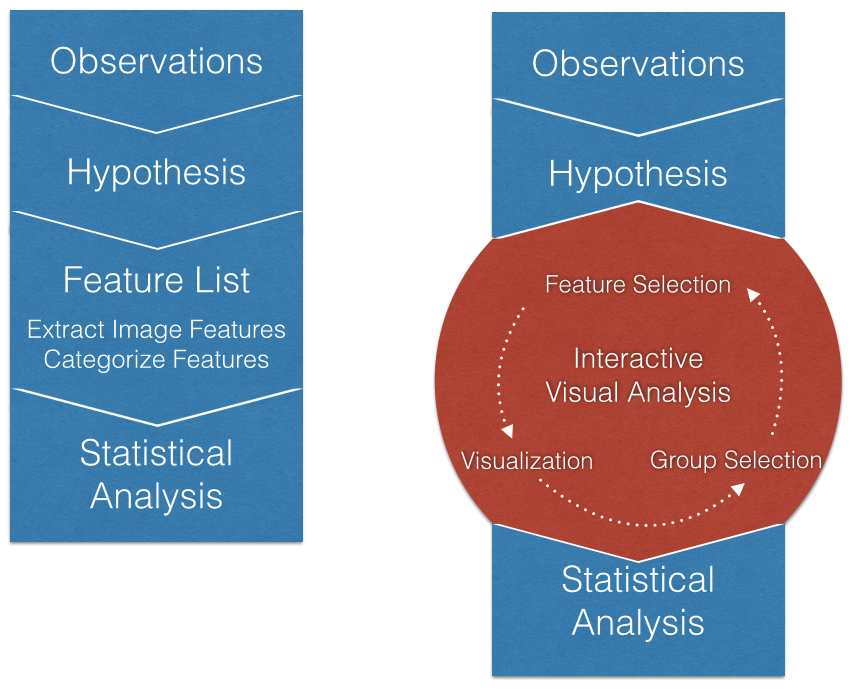
\includegraphics[width=3.0in]{figures/workflow_comparison}
 \caption{
 (a) The standard epidemiology workflow consists of four steps.
 %
 (b) \emph{IVA} tools complement parts of this workflow instead of replacing them.
 %
 The combination of statistical and interactive-driven analysis shows promising potential to unveil information in the data.
 %
 %IVA complements this workflow and is used to elaborate the feature selection.
 %
 We call the iterative red highlighted part \emph{IVA Loop}, described in detail in Figure~\ref{fig:InteractionLoop}.
 %(a) shows the standard epidemiological workflow, (b) the \emph{IVA} supported one. The iterative red highlighted part is called the \emph{IVA Loop} and is described in more detail in Figure~\ref{fig:InteractionLoop}.
 %
 }
  \label{fig:WorkflowComparison}
\end{figure}
The diversity of epidemiology is reflected in the different experts who work at cohort studies, ranging from specialized doctors to medical computer scientists with focus on biometrics, and statisticians.
%
Epidemiologists follow a workflow mainly driven by statistic tools to validate hypotheses about disease-specific risk factors.
%
Following Thew et al. \cite{Thew2009}, the workflow can be characterized as follows:
%
\begin{enumerate}
	\item A hypothesis is derived from observations made by clinicians in their daily routine.
%
	\item A set of features depicting conditions affected by the hypothesis is compiled accordingly.
%
	\item Confounding features are identified and taken into account (for example using stratification).
%
	\item Statistical methods, such as regression analysis, assess the association of selected features with the investigated disease.
%
\end{enumerate}
The workflow is shown in Figure~\ref{fig:WorkflowComparison} (a) and serves as orientation for our approach although it does not consider image data.
%
We focus, on the potential of image data and attempt to support \emph{hypothesis generation}.

\emph{Reproducibility} of results is an epidemiological key requirement.
%
It is difficult to achieve, since many physicians are involved when thousands of test persons are examined and interviewed.
%
Thus, both intra- and inter-observer variability needs to be low for all aspects of a cohort study examination.
%
Longitudinal studies require the acquired features to be comparable for evaluation.
%
%If the data acquisition process changes, an information bias is introduced to the data, hampering inference in and between acquisition cycles.
%
%
Grouping subjects using epidemiological features is essential in cohort studies to allow per-group risk determination.
%
Grouping depends on the underlying hypothesis.
%
Age for example is divided into groups (e.g. in 20 year steps) when investigating its influence.
%
These groups strongly depend on the condition of interest and therefore there is no standard for their categorization.
% --- NEW PARAGRAPH

%
\emph{Relative risks} are determined to detect if a subject is prone to be affected by a certain disease.
%
This includes confidence intervals indicating the certainty of that feature being a risk factor.
%To determine whether a subject is prone to be affected by a certain disease, \emph{relative risks} are expressed through the evaluation of p-values, which indicate statistical significance.
%
Statistical correlations are prone to \emph{confounding}, meaning that the association of two features is influenced by a third feature, which needs to be isolated.
%
A famous example for a confounder is the association between shoe size and mortality, where it can be observed that people with larger shoe size have a smaller life expectation. %than people with small shoe size.
%
The shoe size is actually associated with gender, where women have smaller feet and a longer life expectation.
%
%\add{An extreme form of confounding is called \emph{Simpson's Paradox} \cite{SimpsonsParadox}, where the confounder reverses the observed effect between two features.
%
%A famous example is the Berkeley University gender bias case, where significantly less women were admitted.
%
%Analysis later showed that women applied mostly for strongly restricted subjects and when only looking at acceptance divided by departments there was actually a small bias toward women.
%
%For example, insulin dependent and non-insulin dependent diabetes shows 
%In a famous example, researchers concluded that a newer treatment for kidney stones was more effective than traditional surgery, but it was later revealed that the newer treatment was more often being used on small kidney stones.
%For example, comparing mortality rate of non-insulin dependent 
%When for example surgeons are ranked regarding diseased patients, without including the risk of the surgeries, the results may be distorted.
%

Statistical tools such as \texttt{SPSS}\footnote{Product of IBM; \href{http://ibm.com/software/analytics/spss/}{\texttt{ibm.com/software/analytics/spss/}}} play a major role for analyzing epidemiological data.
%
Graphic data representation is largely used to present results rather than gaining insight.
	
\subsection{Epidemiological Data} \label{EpidemiologicalData}
% \com{Primary Reviewer Feedback: Another weakness is on the data analysis; while there is information about the data within the text (including 2.2, 4.1, and 5.2) I would like to see a section that focuses on the data and the challenges thereof.
% This chapter needs to be enhanced! Maybe own section!}
%
% \com{Bernhard: In Section 2 reichen 1-2 allgemeine Sätze, die typische Probleme der Daten beschreiben.}
% \begin{itemize}
% 	\item \com{OpenRefine erwaehnen? Wurde von uns ja nicht mehr verwendet}
% 	\item \com{"I was unsure which type of Image data you had - a better description and the analysis of the data would help here"}
% 	\item \com{Export from SPSS to CSV/JSON - "How do you ensure the semantics of the data is carried over (e.g. for ordinal data)"}
% \end{itemize}
% \rem{Access to epidemiological data is limited and usually controlled by ethics committees.
% %
% Large studies, such as the SHIP, require written proposals reasoning about each requested features and the expected outcome.
% %
% Since the number of features and modalities is steadily increasing, the epidemiological community is aware of the lack of specialized analysis methods, making an acceptance more likely.
% %
% Due to the high sensibility of the data, all identity-revealing information of a person, such as name or place of residence is anonymized.
% }
% --- PARAGRAPH ---

Epidemiological data are strongly heterogenous and incomplete.
%
Information about medical history and examinations, genetic conditions, geographical data, questionnaire results and image data yield a complex data space for each subject.
%
For ethical or medical reasons some features cannot be gathered for each subject, e.g. women-specific questions about menstrual status or number of born children.
%
Follow-up examinations or questions about conditions such as medications taken after a diagnosed disease also yield features only available for a small amount of subjects.
%

Indicators for medical conditions as well as questions about a subject's lifestyle are often \emph{dichotomous}--they have two manifestations (\emph{Yes} or \emph{No}).
%
Dichotomous data can also be derived by aggregating features to yield only two manifestations (e.g. subjects younger or older than 50 years).
%
Medical examinations comprise categorical (e.g. levels of back pain) and continuous values (e.g. age or body size).
%
\add{Data analysis is usually carried out by calculating correlations,
which is challenging due to the data type heterogeneity.
%
Parameter correlation can also be associated with confounding, which can not be automatically predicted, it has to be judged by a domain expert.
%
Sparse populated features are hard to assess statistically.
%
Too few data samples may distort the real underlying distributions.
%Also, correlation can both be of epidemiological interest but 
}

\paragraph{Image Acquisition.} Imaging techniques involving ionizing radiation for the subject are not suitable for ethical reasons.
%
Therefore, MRI is the main method for collecting cohort study imaging data.
%
The image quality is a tradeoff between accuracy and affordability \cite{Preim2014}.
%
This often yields image resolutions inferior to those of clinical day-to-day practice, which makes their analysis more challenging.
%
%\rem{The equipment used to gather medical image data is not updated or changed during a longitudinal study to ensure comparability in and between acquisition cycles.}

\paragraph{Image Analysis.}
%
Decisions have to be made about \emph{comparison} and \emph{quantification} of image data.
%
Segmentation masks representing the voxels of an anatomical structure would be ideal, since many different key figures, e.g., volume, largest diameter or aspect ratio, can be derived from them.
%
Since reliable and efficient segmentation techniques are not available in general, epidemiologists are forced to measure the data by hand. %, which is a very tedious work with respect to the number of necessary landmarks and the number of subjects.
%
Information derived by landmarks, such as top and bottom point of a vertebra, are by far not as expressive and versatile as segmentation masks describing its whole shape.
%
They are also prone to a high inter-observer variability.
%
%This gains even more importance when analyzing multiple time steps.
%
Morphometric information from landmarks comprises thickness, diameter or length of a structure as well as grey value distribution in an area. %\rem{(for determining the tissue type).}

% Bernhard Paper\\
% - sociodemographic data\\
% - medical data\\
% - pain indicators\\
% - DATA TYPES\\
% 	- dichotomous data\\
% \\

\subsection{The Study of Health in Pomerania (SHIP)}
After the pioneering Rotterdam study (started in 1990), several MR imaging study initiatives were initiated.
%
They slightly differ in clinical focus, acquired data and epidemiological research questions.
%
Starting in 1997 with a cohort of 4,308 subjects, the \texttt{SHIP}, located in Northern Germany, aims to characterize health and disease in the widest range possible \cite{Volzke2011}.
%
Data are collected without focus on a group of diseases.
%
This allows to query the data regarding many diseases and conditions.
%
Subjects were examined in a 5-year time span, continuously adding new parameters including MRI scans in the last iteration \cite{Hegenscheid2009}.
%
%The MRI protocol features many of sequences.
%
% \rem{A second cohort \texttt{SHIP-Trend} was established in 2008.
% %
% The protocols for examining the subjects between \texttt{SHIP} and \texttt{SHIP-Trend} remained the same, making them comparable.
% %
% The overall examination time for each person attending the study is two days.}

% \subsection{Data Analysis Challenges}
% The challenges of analyzing epidemiological data are diverse.
% %
% Risk factors of a disease are rarely limited to one epidemiological feature and most often feature combinations.
% %
% Confounding effects between these features need to be identified and eliminated, which requires large experience of the experts.
% %
% Analyzing large heterogenous feature spaces is difficult due to missing techniques providing \emph{overview visualizations}, forcing epidemiologists to stick to their hypothesis-driven workflow described in Section~\ref{EpidemiologicalWorkflow}.
%
% Another great problem is how image data is analyzed in context with non-image data.
% %
% Epidemiological use of image data is for the most part restricted

% - Missing Data\\
% - Follow-Up Questions?\\
% - grouping essential\\
% - problems when analyzing image data\\
% 	- what are Problems there\\
% 	- how can shape be included?\\
% 	- show image data of multiple subjects
% ---------------------------------------------------------------------------------
% ----------------------------------- Section -------------------------------------
% ---------------------------------------------------------------------------------
\section{Prior and Related Work}

This section describes prior and related work and covers visual analysis 
methods incorporating both image and non-image data. 

\paragraph{Visual Analysis of Image and Non-Image Data.}

Our work is closest to that of Steenwijk \cite{Steenwijk2010}, Turkey \cite{Turkay2013}, and Angelelli \cite{Angelelli2014} and colleagues\add{, who employ multiple coordinated view systems for the analysis of cohort study.}
%
%They employ multiple coordinated view systems for the analysis of cohort study data and demonstrate their approaches based on an aging study \cite{Turkay2013, Angelelli2014} and a cohort of patients suspected of having a special type of rheumatic disease \cite{Steenwijk2010}.

Steenwijk et al. \cite{Steenwijk2010} propose a relational database to organize cohort study data for a visual analysis based on linked views such as parallel coordinates, scatterplots and time plots.
%
Information about medical image data is incorporated via mappers, which extract comparable metrics about the data.
%
Medical image data can be displayed individually for subjects, e.g., for analyzing outliers.
%
\add{While we use a similar approach when analyzing non-image data, our process also includes \emph{overview visualizations} and statistical suggestions of potentially interesting features.}
%

Turkey et al. \cite{Turkay2013} present \emph{hypothesis generation} based on descriptive statistics of the data dimensions.
%
Key figures describing the distribution of data values, e.g., standard deviation and interquartile range, are computed per dimension and analyzed by pairs in a \emph{deviation plot}.
%
%Dimensions can represent non-image data as well as variables derived from image data, e.g., volume of a brain structure.
%
The \emph{dual analysis} of data items and dimensions in multiple linked views led to several hypotheses in analysis sessions with domain experts.
%
%Care must be taken when observing changes in the deviation plot since the resulting hypotheses may impose \emph{overfitting} to the data because the measures highlight only parts of the statistical changes.
Hypotheses based on observations in the deviation plot may impose \emph{overfitting} to the data because the measures highlight only parts of the statistical changes.
%
\add{Our approach uses information extracted from the segmented image data (such as 3D meshes) and variable associations with non-image epidemiological factors.}

Angelelli et al. \cite{Angelelli2014} focus on a suitable data organization for the interactive visual analysis of heterogeneous cohort study data.
%
%\rem{They propose a data-cube based model able to handle partially overlapping data subsets during the interactive visualization.}
%
Brain image data was integrated into the analysis by first, segmenting brain regions and tracking neural pathways and then, deriving attributes from both, e.g., volume and fractional anisotropy.
%
The data-cube model facilitates the seamless integration of heterogeneous image-based and non-image data.
%
A multiple coordinated view framework linked spatial and non-spatial data views.
%
%The approach is a demonstrated by a case-study analysis of selected aspects of brain connectivity.
% --- Steffens Fazit ---
%
\add{Our integration of image data into the analysis is similar to the work of Steenwijk \cite{Steenwijk2010} and Angelelli \cite{Angelelli2014} and colleagues.
%
While they offer a single spatial view for visualizing image-based information of one subgroup of the cohort, we provide multiple, small views showing the information of subgroups and its respective deviation from the entire cohort.}
%
%\rem{We also integrate the data-driven definition of subgroups using clustering, statistically-based suggestions of potentially interesting features, and adaptive feature visualization.} %tailored to epidemiological data, e.g., a mosaic plot for the frequent categorical variables.
% %
% %Another unique characteristic is our web-based implementation and the integration of D3.js.
% %
% %The latter offers an extensive set of information visualization plots, which are at the disposal of our system.
% %
% --- / Steffens Fazit ---

Gresh et al. \cite{Gresh2000} proposed \texttt{WEAVE}, one of the first systems which concurrently analyzed medical image and non-image data using linked views.
%
Blaas et al. \cite{Blaas2007} presented a similar system, which also analyzed medical image data and variables derived from them using views from the feature and physical space.
%
Both works are restricted to the analysis of one case at a time and to non-image data with a unique spatial reference, e.g., voltage simulated across the heart muscle.
%
In epidemiology, multiple cases must be concurrently investigated and non-image data often lacks a spatial reference, such as gender and age.
%
% \com{\textbf{Reviewer 1}: The related work section includes merely a set of related tools. I would have liked to see a more comprehensive section that discusses the previous related work in more detail and describes why they are important and relevant to this work and how your work differs or improves upon theirs.\\
% %
% Quality: The work contains many references. But there are potentially some missing; e.g, the framework talks about utilizing multiple coordinated views (although the details of what is actually linked is vague) and therefore cited papers such as Baldonado's work in AVI 2000, or Roberts 2007 on Coordinated multiple views, or Weaver's Cross-filtered Views for multidimensional visual analysis 2010 should be cited. The paper really proposes a framework; however it was unclear how this was implemented into the presented system. Therefore this should be improved.\\\\
% %
% \textbf{Reviewer 2}
% - I would suggest to also cite the original Generalized Pairs Plot and
% not only the adaptation as GPLOMS [21]: J. W. Emerson and W. A. Green.
% gpairs: The Generalized Pairs Plot, 2012. R package version 1.1.\\
% %
% - A related process model for Visual Analytics that focuses on hypotheses
% and models: T. Lammarsch, W. Aigner, A. Bertone, S. Miksch, and A. Rind,
% “Towards a Concept how the Structure of Time can Support the Visual
% Analytics Process,” in Proceedings of International Workshop on Visual
% Analytics (EuroVA 2011) in conjunction with EuroVis 2011, Goslar,
% Germany, 2011, pp. 9–12.\\
% %
% - VISITORS is related work in visualization of medical variables of
% cohorts: D. Klimov, Y. Shahar, and M. Taieb-Maimon, “Intelligent
% visualization and exploration of time-oriented data of multiple
% patients,” Artificial Intelligence in Medicine, vol. 49, no. 1, pp.
% 11–31, May 2010.\\
% %
% - another, forthcoming related paper: P. Angelelli, S. Oeltze, C. Turkay,
% J. Haasz, E. Hodneland, A. Lundervold, A. Lundervold, B. Preim, and H.
% Hauser, “Interactive Visual Analysis of Heterogeneous Cohort Study
% Data,” IEEE Computer Graphics and Applications, vol. Early Access
% Online, 2014.\\\\
% %
% \textbf{Reviewer 3}
% What the prior work section needs at the end is a paragraph stating how their work differs from the work they summarise i.e. it uses more non-image data than Turkay and uses different visualisations, and more importantly differentiation from Steenwijk et al’s very similar work (saying they use a different meaning for the word “cohort” does not seem justification enough, given the large overlap), only then can we be sure there is a novel contribution here.}

% ------------------ OLD SECTION ---------------------
% \add{%Multiple coordinated views are appropriate for analyzing epidemiological data, because it suits Baldonado et al's \emph{Rule of Diversity} \cite{Baldonado2000}.
% %
% This section describes prior and related work and covers visual analysis methods incorporating both image and non-image data.
% %
% %We divide these section accordingly and also present lessons learned and from each publication.\\
% }
% %Designing a visualization, which conveys all data aspects equally, is challenging.
% % --- PARAGRAPH ---
%
% Given the number of features of epidemiological data sets and their different manifestations, the strength of different visualization techniques needs to be combined \cite{Buja91, Konyha2009}.
% %
% The principal component analysis (PCA) and similar techniques are able to reduce the dimensions by extracting most expressive components, but make the influence of each variable hard to convey.
% \\\\
% %Their focus on \emph{hypothesis generation} using parallel assessment of multiple data features makes the work of Turkay et al. closest to ours albeit our emphasis on processing models derived from medical image data segmentation and variables with categorical manifestations \cite{Turkay2013}.
% Turkay et al. \cite{Turkay2013} focus on \emph{hypothesis generation} using parallel assessment of multiple data features makes their work closest to ours albeit our emphasis is on processing models derived from medical image data segmentation and variables with categorical manifestations.
% %
% Their methods aim to amplify a hypothesis generation process for analyzing data of a Norwegian aging study.
% %
% Statistical measures of continuous features, such as mean, standard deviation, skewness, or inter-quartile range, are used to create \emph{dimension plots}. %that make them comparable with respect to the derived descriptive measures, such as voxel number of a segmented structure.
% %
% These transform dimensions into data points and make them comparable with respect to the derived descriptive measures, making them comparable.
% %
% %This not only allows for comparing all continuous variables in a single plot but make their distribution change comprehensible.
% %
% %This requires a good descriptive measure which captures the kind of change the user is interested in or which reflects unexpected data behavior.
% %
% %The technique was applied to features obtained by segmenting the brain into 45 parts and measure the voxel number, volume and properties of the intensity values.
% %
% The method is strongly dependent on the descriptive measures of the epidemiological factors.
% %
% %\emph{Over-fitting} of hypotheses to the data may be imposed  is a danger pointed out by the authors when hypotheses to the data based on observations of changes in these plots the measure highlights only subsets of statistical changes.
% Hypotheses based on observations of changes in these plots may impose \emph{overfitting} to the data because the measures highlight only parts of the statistical changes.
% %
% %Our approach sticks more to the information extracted from the segmented image data and variable associations with non-image epidemiological factors.
% \add{Our approach uses information extracted from the segmented image data (such as 3D meshes) and variable associations with non-image epidemiological factors.}
% % Disadvantage - Nur 2 abgeleitete Variablen sichtbar, schlecht mit anderen Variablen in Verbindung zu bekommen (müsste jedoch auch gehen) - viele Dinge gehen durch die Abstraktion aber auch flöten!
%
% \paragraph{Visual Analysis of Image and Non-Image Data.}
% %\add{One major focus is the connection of image and non-image data.}
% %TODO aus Steenwijk: Visual data analysis combining multi-dimensional single patient medical data with real-time linked scatter plots and parallel coordi- nates representations was first investigated in the WEAVE system of Gresh et al. [14]. A number of aspects with regards to the specifi- cation of this kind of focus+context visualization were formalized by Doleisch et al. [8].
% Gresh et al. \cite{Gresh2000} proposed \texttt{WEAVE}, one of the first systems which concurrently analyzed medical image and non-image data using linked views.
% %
% %\add{The functionality is limited to project spatial related data to surface renderings of the image data and use By projecting surface models presented in 3D views to information visualizations, such as scatterplots, the authors were to support medical resea}
% %
% Blaas et al. \cite{Blaas2007} presented a similar system, which also analyzed medical image data and variables derived from them using views from the feature and physical space.
% % From Blaas2007 - Tasks:
% %- Investigating combinations of features for finding spatial separations of point sets in physical space (segmentation)
% %- Classification of feature point sets (pattern classification)
% %- Finding clusters, patterns, and relations in the data
% \add{The parameter in both paper are part of the spatio-temporal domain and have a colocation in the image data, making it possible to plot them onto the image data representation to investigate interesting combinations.
% %
% Epidemiological features often don't have an exact spatial location in the image data.}
% %
% Steenwijk et al. \cite{Steenwijk2010} employ a relational database to organize the data for visualizing subject data using linked views such as parallel coordinates, scatterplots and time plots.
% %
% \add{Information about medical image data is incorporated via mappers, which extract comparable metrics about the data.
% %
% Medical image data can be displayed individually for subjects, e.g. for analyzing outliers.
% %Display of medical data is possible for single subjects, for example to look at outliers.
% %
% While we use a similar approach when analyzing non-image data, our process also includes \emph{overview visualizations} and statistical suggestions of potentially interesting features.}
% ------------------ / OLD SECTION ---------------------
\paragraph{Visual Analysis of Heterogenous Non-Image Data.}
Zhang et al. \cite{Zhang2012} provide a web-based system for analyzing subject groups with linked views and batch-processing capabilities for categorizing new subject entries into the data set.
%
Their understanding of a cohort differs from the understanding of the term in an epidemiological context by denoting every parameter-divided subject group as individual cohort.
%
\add{Due to the short paper length, detail is missing on the data type and their algorithm of identifying similar subjects works or what and if they employ statistical measures.
%
We employ the idea of adding features via drag and drop into a canvas area.}

Generalized Pairs Plots (\texttt{GPLOM´S}) are an information visualization technique comparing heterogenous features pairwise using a plot-matrix grouped by type \cite{GPLOMS, Francois2013}.
%
They are useful to gain an overview over numerous variables and their distributions.
%
Histograms, bar charts, scatterplots and heat maps are used to visualize variable combinations with regard to their type.
%
\add{The resulting matrix provides a \emph{overview visualization}, but requires a lot of screen space for many features (127 in our application scenario).}
%
%Brushing, linking and filtering are feasible with \texttt{GPLOMS}, but have limitations such as making only one category brushable at a time.
%
%We applied this technique to our data and it shows promising potential for simultaneously visualizing many different variables. %but does not fit in the scope of this paper.
%
\add{We incorporate the idea of adaptive type-dependent visualizations.}
%\add{The inspiration on the chosen visualization techniques stems from this publication.}
%
Dai et al. \cite{Dai2005} explored risk factors by incorporating choropleth maps of epidemiological features (e.g., mortality rates in a region) with parallel coordinates, bar charts and scatterplots with integrated regression lines.
%
Their findings yielded a \emph{Concept Map}, which linked cancer-related associations via graph edges.
%
\add{While their goal to identify possible risk factors using socio-economic and health data are similar to ours, they focus on iteratively refining defined hypothesis and also focus on geographical data.
%
We employ the use of small multiples in this publication for incorporating heterogenous data types for comparability.}
%
Chui et al. \cite{Chui2011} visualized associations in time-dependent epidemiological data using time-series plots highlighting risk factor differences in age and gender.
%
\add{%The connection of time series plots with histograms and heat maps allows for fast insight into complex relationships and 
While the works shows, how different visualization modalities provide insight into these data sets, it focuses on the time aspect, which is not present for our data.}
%
% \paragraph{Commercial Data Visualization.}
% Commercial systems such as \texttt{Tableau}\footnote{Owned by Tableau Software; \href{http://tableausoftware.com}{\texttt{tableausoftware.com}}} or \texttt{Spotfire}\footnote{Owned by TIBCO; \href{http://spotfire.tibco.com}{\texttt{spotfire.tibco.com}}} provide a rich user interface that enables a Visual Analytics approach.
% %
% With little effort, linked views can be created, but the data processing possibilities, such as derivation of new variables or the 3D rendering capabilities, are very limited.
% %
% These systems with their origin in business intelligence applications do not support epidemiological workflows well, in particular workflows that also consider medical image data.
% Image Data
% \paragraph{Visualizing Image Data.}
\paragraph{Visualizing Shape Variance.}
Comparing tissue between many subjects requires shape variance visualizations.
%
Caban et al. \cite{Caban2011} investigated the suitability of variance visualizations of shape distribution models and concluded that users favor spherical glyph representations over deformation grids and likelihood volumes.
%
The distribution of shapes in a space derived from a PCA is plotted by Busking et al. \cite{Busking2010a} in a 2D-projected plane of the space.
%
Interpolated views can be created by the user in a separate view as well as comparisons in a contour view.
%
Interpolation is carried out by mesh morphing.
%
The distance to the mean shape is color-coded.
%Differences between structures are highlighted using color mapping of the difference to the mean shape, but is rather hard to recognize due to small renderings of each subject in the shape-space.
%Via mesh morphing interpolated views can be created by the user in a separate view as well as comparisons in a contour view.
%
We incorporate the idea of combining 3D shape rendering with information visualization techniques.
%
\add{Applying our data sets to this technique yielded a cluttered shape space due to the many subjects.
%
The data needs to abstracted or summarized in order to work in this context.}
%
Hermann et al. \cite{Hermann2014} identify local deformation changes by investigating shape-related differences on rodent mandibles.
%
User-specified regions of interests are mapped to associated anatomic covariation using tensor visualization.
%Anatomic covariation induced by user input is displayed using tensors 
%Specifying a change in shape of a certain area by the user shows how other parts of the model would react using covariance tensors.
%Covariance tensors indicate how a model is deformed when the user given a user specified deformation.
%The user specifies a deformation of interest and showing corresponding changes in the shape using covariance tensors.
%
This method enables rapid hypotheses validation and was able to reproduce textbook knowledge.
%
%By plotting p-values in ventricle surfaces, Chou et al. were able to map disease-associated values directly on a 3D tissue representations \cite{Chou2009}.
%
\add{This requires a geographic colocation of associated features.}
%

% *********************** Our own Work ***********************
% Prior Work
\paragraph{Prior Work.}
Klemm et al. \cite{Klemm2013VMV} visualized lumbar spine variabilities based on a semi-automatic shape detection algorithm of 490 participants of the \texttt{SHIP-2} cohort.
%
Hierarchical agglomerative clustering divided the population into shape-related groups.
%
As proof of concept, a relation between the size of the segmented shape and measured size of the subjects was shown.
%
This work focuses on incorporating these derived data as new features of the overall data set, making it possible to include it into the hypothesis validation and generation process.
%
When applying clustering techniques to the non-image data it was found that \texttt{k-Prototypes} and \texttt{DBSCAN} are appropriate in the epidemiological context, but is strongly dependent on the chosen variables and distance measure \cite{Klemm2014BVM}.
%
Niemann et al. \cite{Niemann2014} presented an interactive data mining tool for the assessment of risk factors of hepatic steatosis, the fatty liver disease.
%
Association rules created by data mining methods can be analyzed interactively with their tool and highlight potentially overlooked features.
%
\add{We combine the idea of suggesting potentially interesting features by adding them to the \emph{IVA}-workflow in order to amplify hypothesis generation.}
% *********************** / Our own Work ***********************

\paragraph{Interactive Visual Analysis.}
% Interactive Visual Analysis - Steffens Paper
The strength of the \emph{IVA} approach described in the next section is its versatility with respect to the application field \cite{Konyha2009}.
%
Oeltze et al. proposed a multiple coordinated view approach for the analysis of medical perfusion data \cite{Oeltze2007} and biological multi-channel fluorescence microscopy data \cite{Oeltze2011}.
%
The approach is restricted to the investigation of a single subject at a time.
%
%While we take similar steps when analyzing the data such as employing statistical tests, our data is mostly independent from the medical image data and is not describing it. %--except the variables derived the segmentation model itself.
% --- PARAGRAPH --- 

Lammarsch et al. \cite{Lammarsch2011} provided a workflow and terminology definition of Visual Analysis techniques.
%
They define a model as a representation of system entities, phenomena and processes and hypothesis as models whose outcomes are not compared with real-world data (\emph{validation}).
%
The VA-process is also reflected in our \emph{IVA}-Loop.
% --- PARAGRAPH ---

Baldonado et al. \cite{Baldonado2000} presented rules for designing multiple coordinated views.
%
They point out the cost-benefit-tradeoff introduced by the cognitive overhead by mentally connecting multiple views over more complex single views. %introduced by tasks, such as view comparison or context switching.
%
Weaver et al. \cite{Weaver2010} extracted guidelines for cross-filtering multiple views by incorporating \emph{views} mapping data to visual elements, \emph{brushes} for selecting these elements and \emph{switches} for linking brushing results between \emph{views}.
%
Our system follows the same rules for selecting subject groups, but our goal is to judge feature relations and potential outcomes.
\\\\
%Related work focused on epidemiological data often deals with time-dependent data, hypothesis generation by guidance through parameter suggestions is seldom.
\add{The uniqueness of the \emph{IVA} workflow applied to image-based cohort study data compared to the discussed work are threefold.
%
(1) We incorporate 3D models abstracting shape information (e.g. for the spine) fused with non-image data visualizations, allowing to analyze local physiological changes related to non-image parameters.
%
(2) Epidemiologists already have an well established workflow for statistically validating hypothesis. 
%
Therefore, we focus on hypothesis generation by discovering new relationships associated with shape information.
%
(3) Overview visualizations using statistical abstractions aim to provide an unbiased feature relationship assessment.
}

%\section{Interactive Visual Analyis in Cohort Study Data}
\section{Image Centric Cohort Study Data in Interactive Visual Analysis Context} \label{Image Centric Cohort Study Data in Interactive Visual Analysis Context}
We described the epidemiological workflow and emphasized the reproducibility and statistical integrity (recall Subsection~\ref{EpidemiologicalWorkflow}).
%
%Figure~\ref{fig:WorkflowComparison} (a) shows this workflow as a consecutive series of steps.
%
%Introducing the \emph{IVA} principle to the epidemiological domain aims to compensate its weaknesses rather than replacing the existing workflow.
Introducing the \emph{IVA} principle to the epidemiological domain aims to compensate the weaknesses of the existing workflow, rather than replacing it (recall Fig.~\ref{fig:WorkflowComparison}).
%
In the current state, the workflow treats the data like a black box.
%
Statistical tests on features associated to a hypothesis yield a value for deciding whether the data supports the hypothesis.
%
Features not included in the analysis may potentially support the chosen hypothesis by discriminating the population in the expected way, but are not highlighted.
%
This becomes even more important when the workflow is adapted to the analysis of the medical image data, where
domain experts annotate landmarks tediously to derive measures, such as diameters.
%
This leaves out the majority of information in the image data by abstracting it to single values.
%
%It is easily possible that omitted information would heavily influence the result.
%
Considering more complex parts of the data would make those results more trustworthy and also could identify possible anatomical confounders--an epidemiolgical research result in itself.
\\\\
\emph{IVA} tries to illuminate the black box by making the domain experts part of an iterative feature selection process (see Fig.~\ref{fig:WorkflowComparison} (b)).
%\emph{IVA} tries to illuminate the black box by making the domain experts part of an iterative feature selection process, which is shown in Figure~\ref{fig:WorkflowComparison} (b) as part of the epidemiological workflow.
%
It also aims to project back into the hypothesis formulation step to amplify hypothesis generation.
%
This has to be handled with care, since \emph{overfitting} of expectations to the data is an imminent danger \cite{Turkay2013}.

\paragraph{Domain and Range Variables. }
In the \emph{IVA} context, data are characterized by a combination of independent variables, such as space and/or time, and dependent variables, like temperature or pressure.
%
Two kinds of views are employed to inspect the data:
\begin{itemize} 
	\item \emph{physical views} \cite{Oeltze2013}, such as direct volume rendering, show information in the context of the spatio-temporal observation space \cite{Oeltze2007}, while
	\item \emph{attribute views}, such as scatter plots and parallel coordinates, show relationships between multiple data attributes.
\end{itemize}
Transferred to epidemiological data, the residential area of cohort subjects could be interpreted as \emph{space}, the different assessment cycles of a longitudinal study as \emph{time}, and the image and non-image data as \emph{dependent variables}.
%
Our current work neglects geographical and temporal aspects.
%
Instead we employ a abstract model and consider the subjects as living in a joint image space where each of them is represented by a segmented organ or structure.
%
For instance, the lumbar spine is segmented over all subjects and all lumbar spines are co-registered spanning a joint space.
%
Then, two types of dependent variables exist: the socio-demographic data and medical examination results, and variables derived from the segmented structures, e.g., spinal curvature or misalignment of the vertebrae.
% \begin{enumerate}
% 	\item the socio-demographic data and medical examination results and
% 	\item variables derived from the segmented structures, e.g., spinal curvature or misalignment of the vertebrae.
% \end{enumerate}
An alternative of the image space would be the shape space generated by extracting the major modes of variation from all segmentation results \cite{Busking2010a}.
%
Based on our abstract model, the three analysis patterns of \emph{IVA} can be employed.

\paragraph{Local Investigation.} Refers to the inspection of dependent variables with respect to subsets of the image or shape space.
%
For instance, the epidemiologist selects several lumbar spines with a common characteristic in the image or shape space and inspects the associated dependent variables in an attribute view \cite{Hermann2014}.
%
The selection step requires dedicated interaction techniques for defining a subset.
%
Alternatively, derived shape-related variables opposed in an attribute view or automatic techniques for shape clustering may be employed \cite{Klemm2013VMV}.
%
Clustering algorithms can be used to investigate associations between shape groups and other non-image variables.
%
Analysis of outliers can indicate segmentation errors or a group of subjects sharing a pathology.

\paragraph{Feature Localization.} Refers to the search for structures in the image or shape space with a defined characteristic.
%
The epidemiologist may be interested in all female subjects with lower back pain and wishes to see the corresponding spines in a physical 3D view.

\paragraph{Multivariate Analysis.} Refers to an investigation of multi-variate properties of the dependent data by specifying a feature in one attribute view while analyzing the value distribution with respect to other variables in other attribute views.
%
Epidemiologists may define a feature in a scatter plot of the body mass index (BMI) and age to inspect the result in a histogram of body height.
%
These associations may also be summarized using pivot tables which are widely used in epidemiology.

\subsection{Data Preprocessing} \label{Data Preprocessing}
%A number of transformations are carried out in the data preprocessing stage.
%Transformation operations on the data to prepare it for an \emph{IVA} system are denoted as data preprocessing.
\paragraph{Non-Image Data. }
%
%Multimodal features require different techniques.
%
Data obtained using questionnaires or medical tests are often stored using statistical packages such as \texttt{SPSS}, which have a proprietary data format. %with limited export capabilities.
%
Exporting the data in the respective tool to a CSV file and then converting it to file types that are easily manageable, such as JSON, makes it readable for modern programming languages.
%
%This can be achieved by using data wrangling tools such as \texttt{OpenRefine}\footnote{Developed by Google, Open Source; \href{http://openrefine.org}{\texttt{openrefine.org}}}, which also validate the data (find missing data, clean up bad formatting, transform scales).
%
A data dictionary stores information about each manifestation of a feature.
%
Detailed description of data variables, its meaning as well as unit of measurement are stored as a lookup table.
%
%Exporting the data dictionary, which stores information about each manifestation of a feature, is also an important step to get a detailed description of data variables and the meaning and unit of measurement of their values.
%
Missing data are denoted using error codes indicating their cause ranging from ethical to medical and personal issues (recall Subsection~\ref{EpidemiologicalData}).
%The reasons for missing data have a wide range from ethical to medical and personal issues.
%
%Therefore, these are also included as error codes which have to be marked as such in the data dictionary.
\paragraph{Image Data. }
Information about anatomical structures, such as diameter or volumes, is extracted from the image data.
%
This is either done manually by experts setting landmarks or by a (semi-)automatic detection, registration and segmentation.
%
These algorithms have to deal with a large inter-subject variability of the anatomical structure \cite{Preim2014}.
%
In principle, model-based approaches are effective for detection \cite{Rak2013} and segmentation \cite{Gloger2010}. %\cite{Gloger2010, Gloger2012}.
%
If a segmentation yields only binary masks separating the structures, algorithms such as \emph{Growing and Adaptive Shapes} can be applied creating a surface grid where each point is comparable throughout the population \cite{Ferrarini2007}.
%
Grey value comparison is used to measure the quantity of fat, water, and--application-specific--the iron content (liver) or the distribution of grey and white brain tissue.
%
Morphometric features are derived to allow for statistical comparison of the tissue, which incorporates mostly positions, diameters, volumes and relative distances and alignment to other structures.
%-------------------------------- Figure --------------------------------
\begin{figure}[htb]
 \centering
 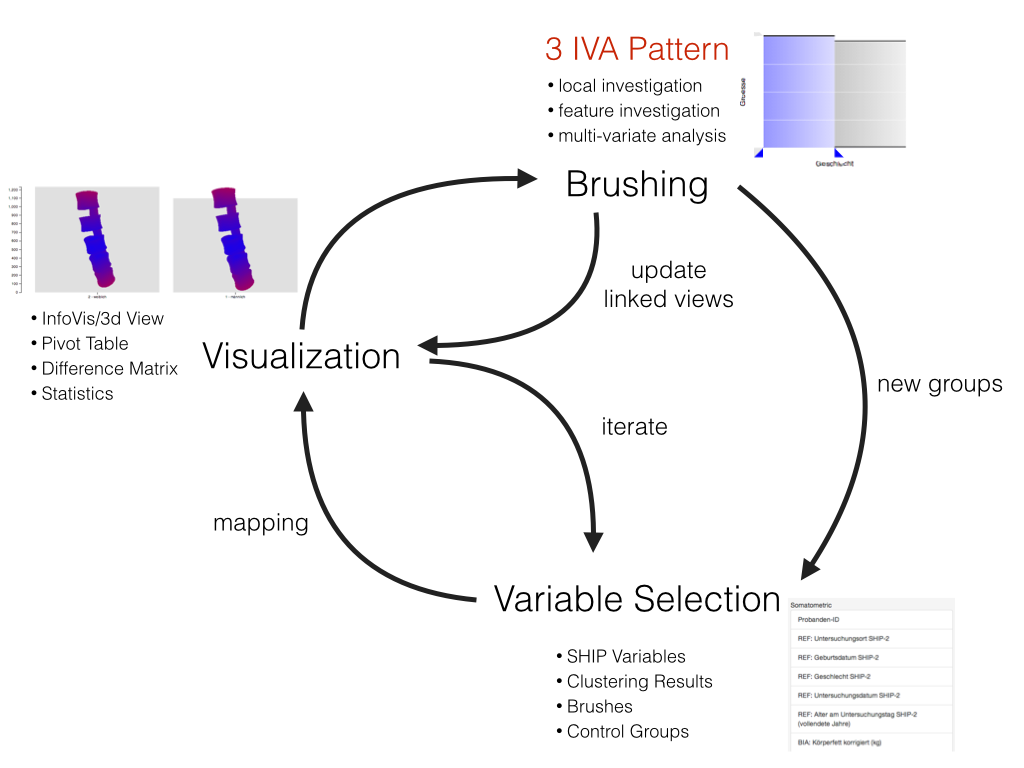
\includegraphics[width=2.0in]{figures/InteractionLoop}
 \caption{Detailed \emph{IVA Loop} as extension from Figure~\ref{fig:WorkflowComparison}.
 %
 Usually starting with a selection of a feature of interest (user-driven or via data mining techniques), the data are mapped using a visualization technique appropriate for the selected data types.
 %
 The data are visualized in the range and domain space, which can be brushed, yielding new groups, to be investigated using further features.
 %
 Note that adjacent steps are directly connected via feedback loops, allowing for an iterative refinement and giving as much freedom to the user as possible.}
 \label{fig:InteractionLoop}
\end{figure}
%------------------------------ / Figure --------------------------------
\subsection{Analysis Workflow}
%-------------------------------- Figure --------------------------------
\begin{figure*}[htb]
 \centering
 %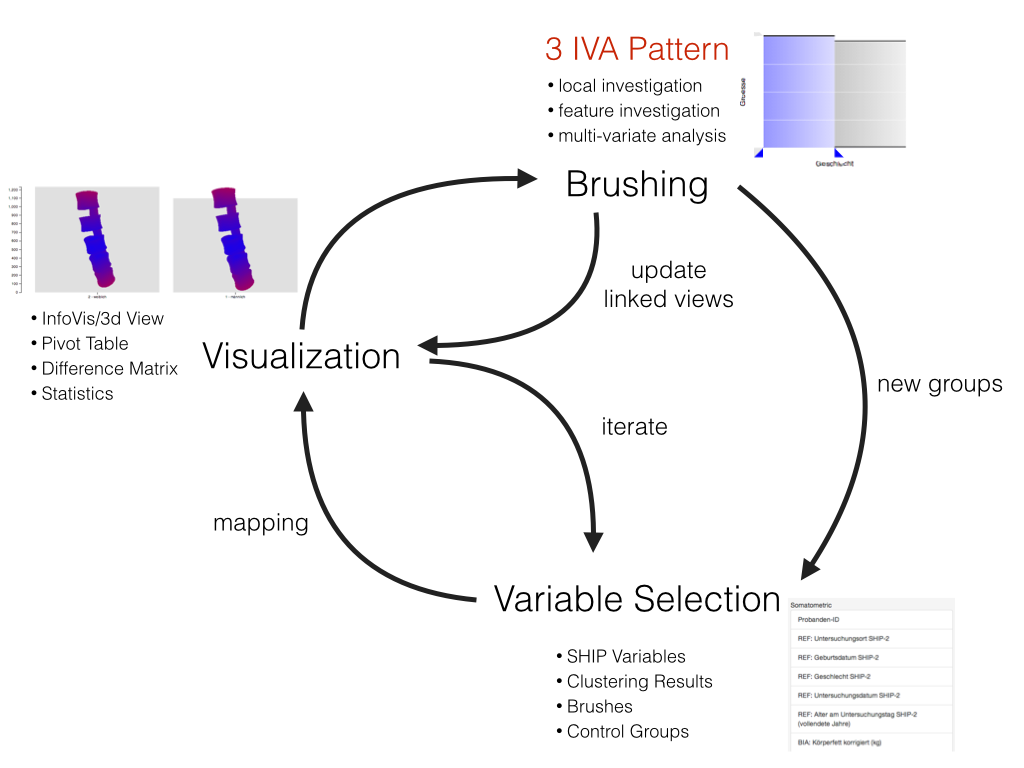
\includegraphics[width=1.5in]{figures/InteractionLoop}
 % 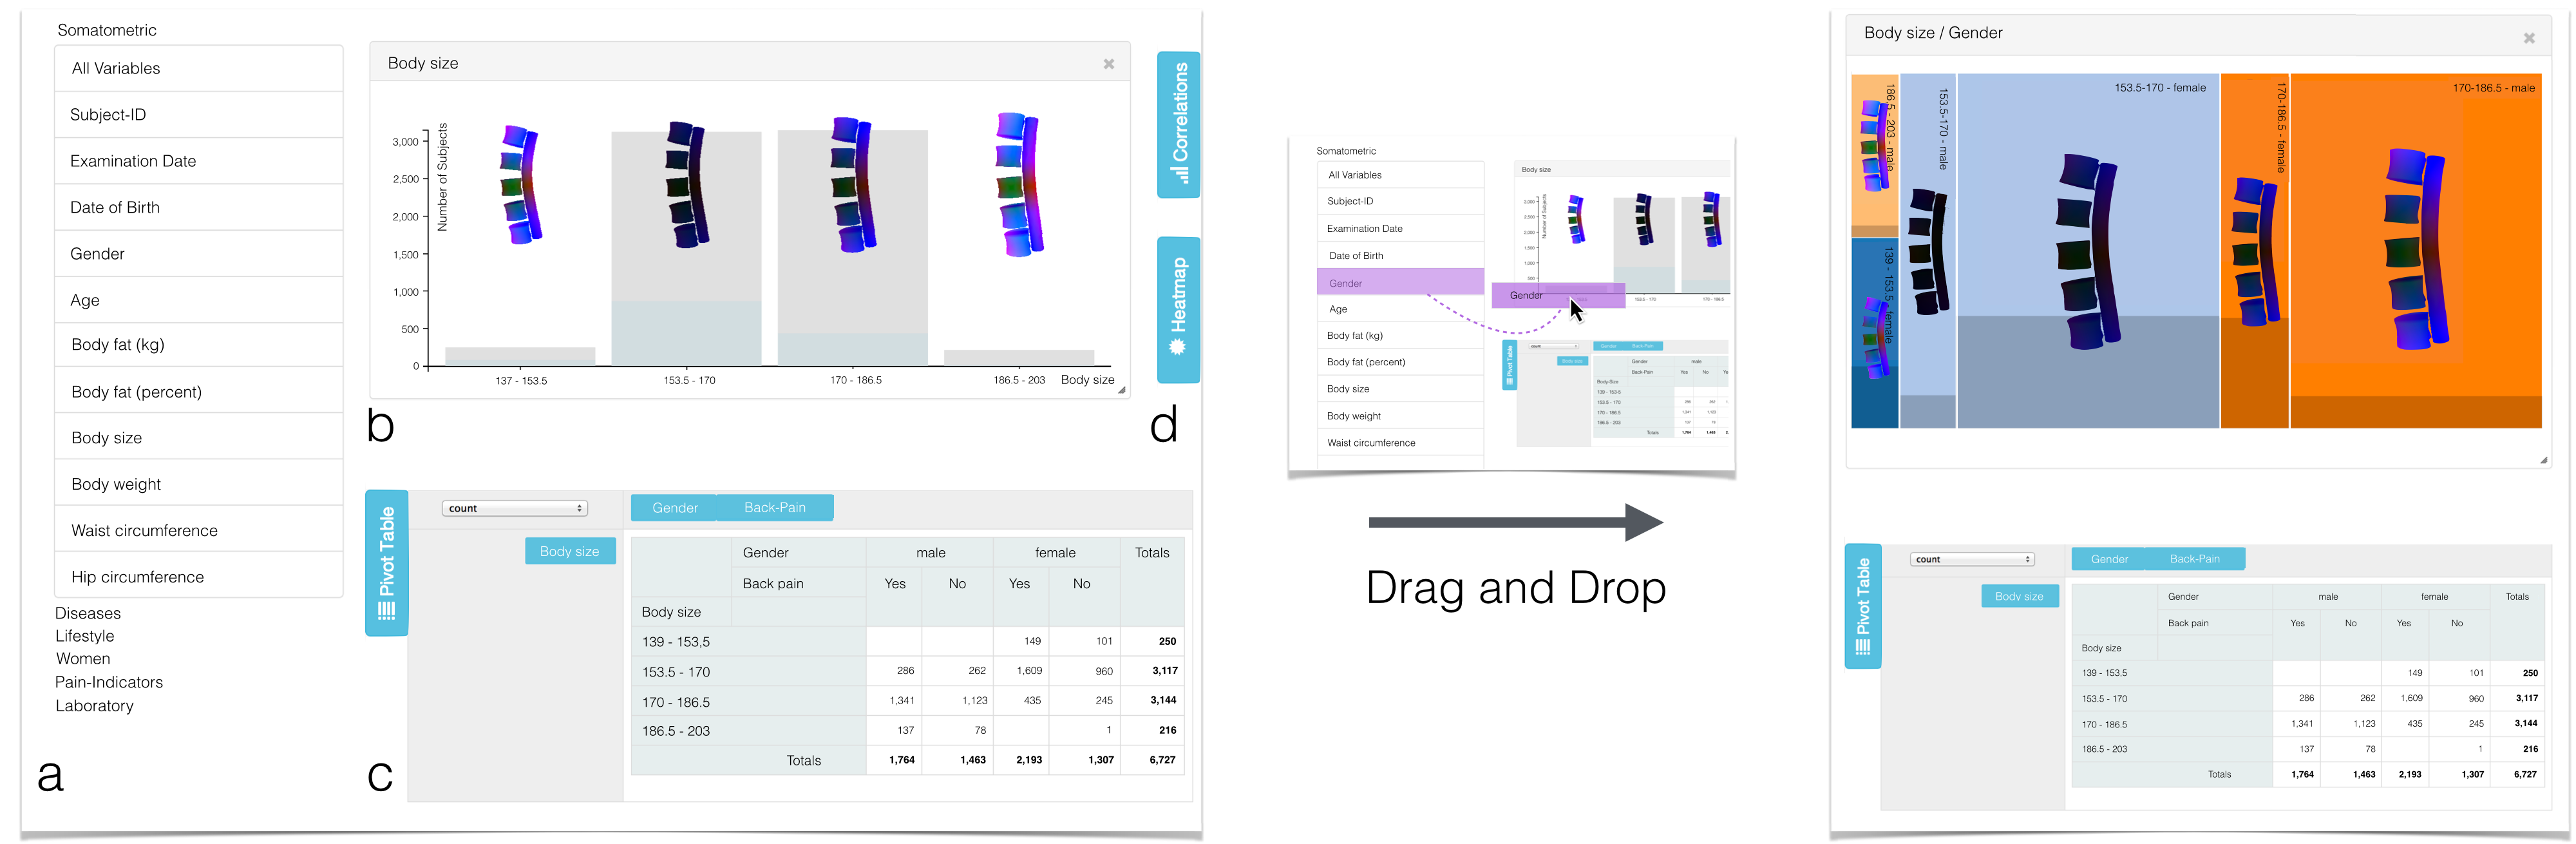
\includegraphics[width=3.5in]{figures/visualization}
 %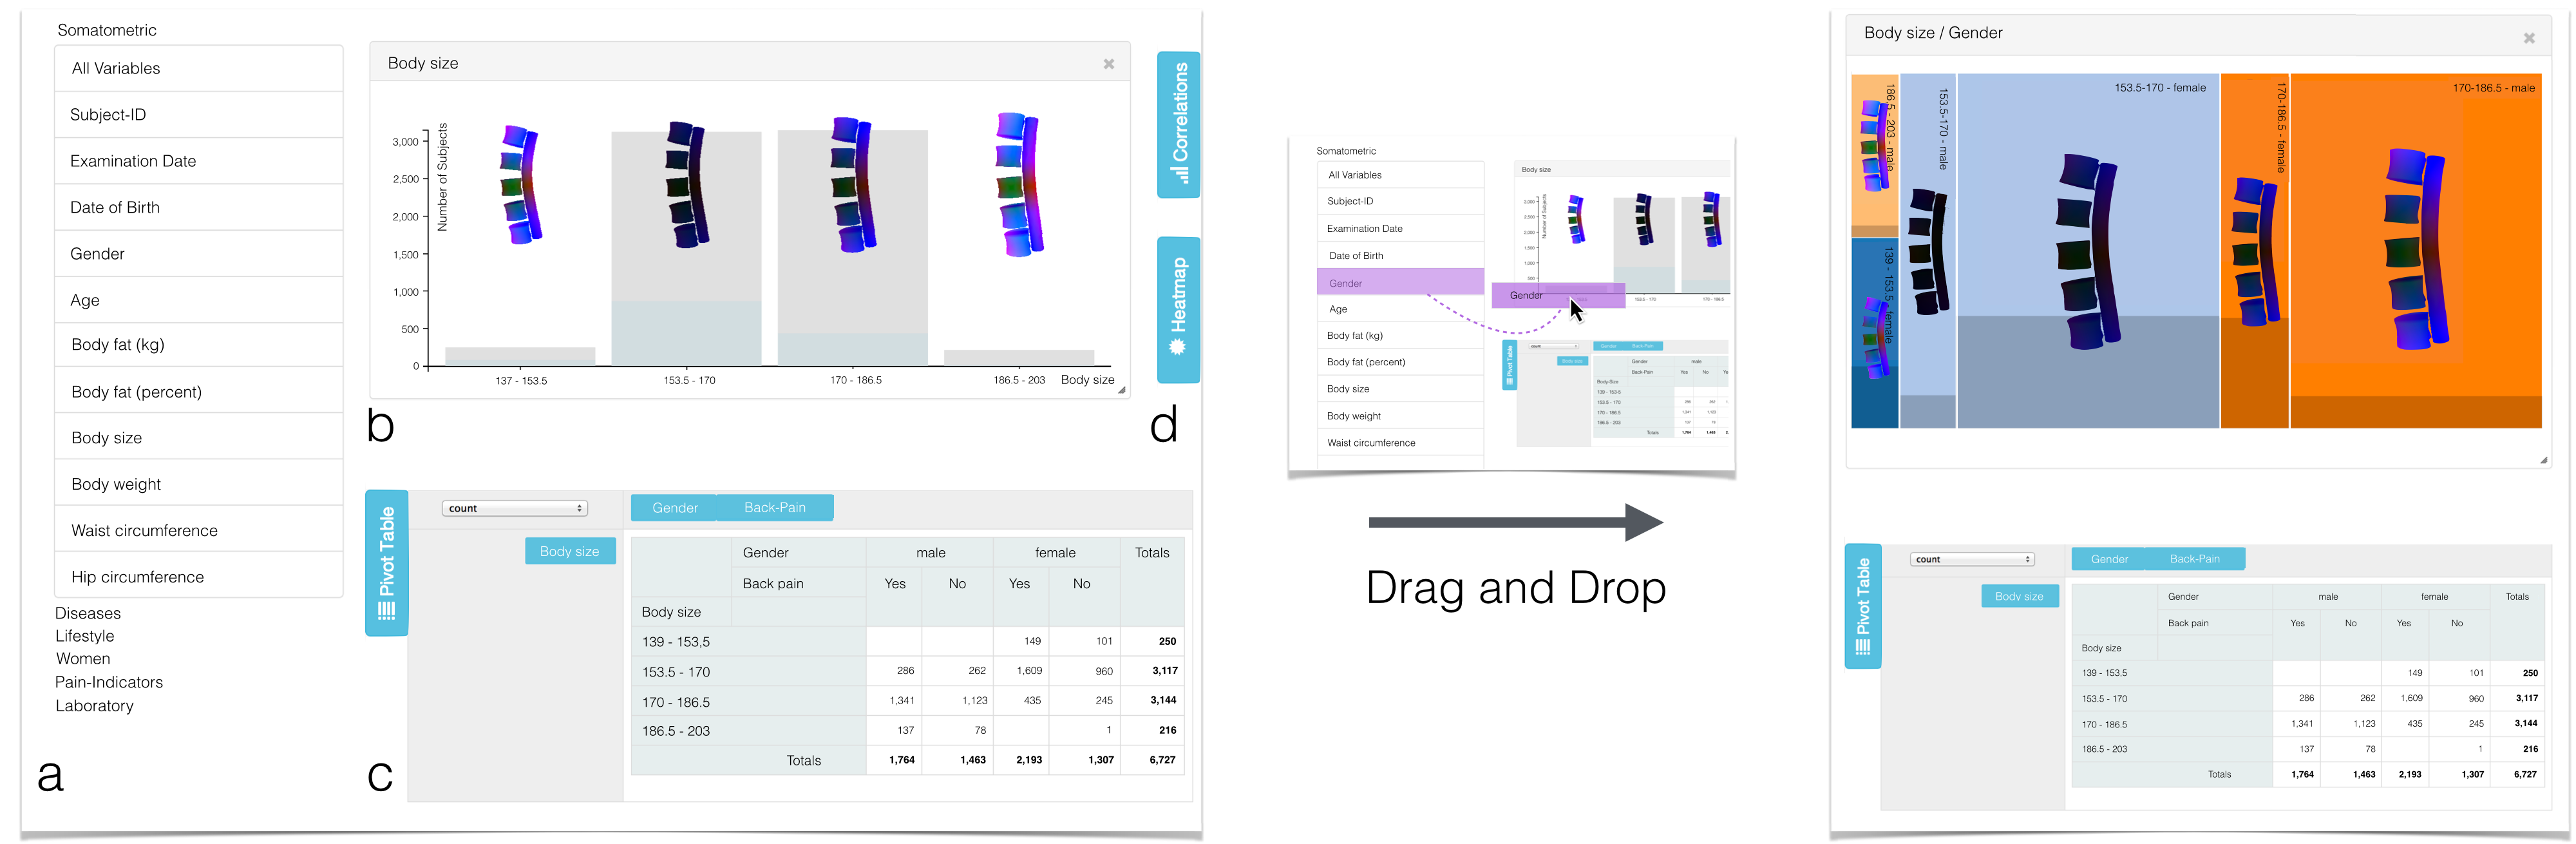
\includegraphics[width=1\textwidth]{figures/visualization}
 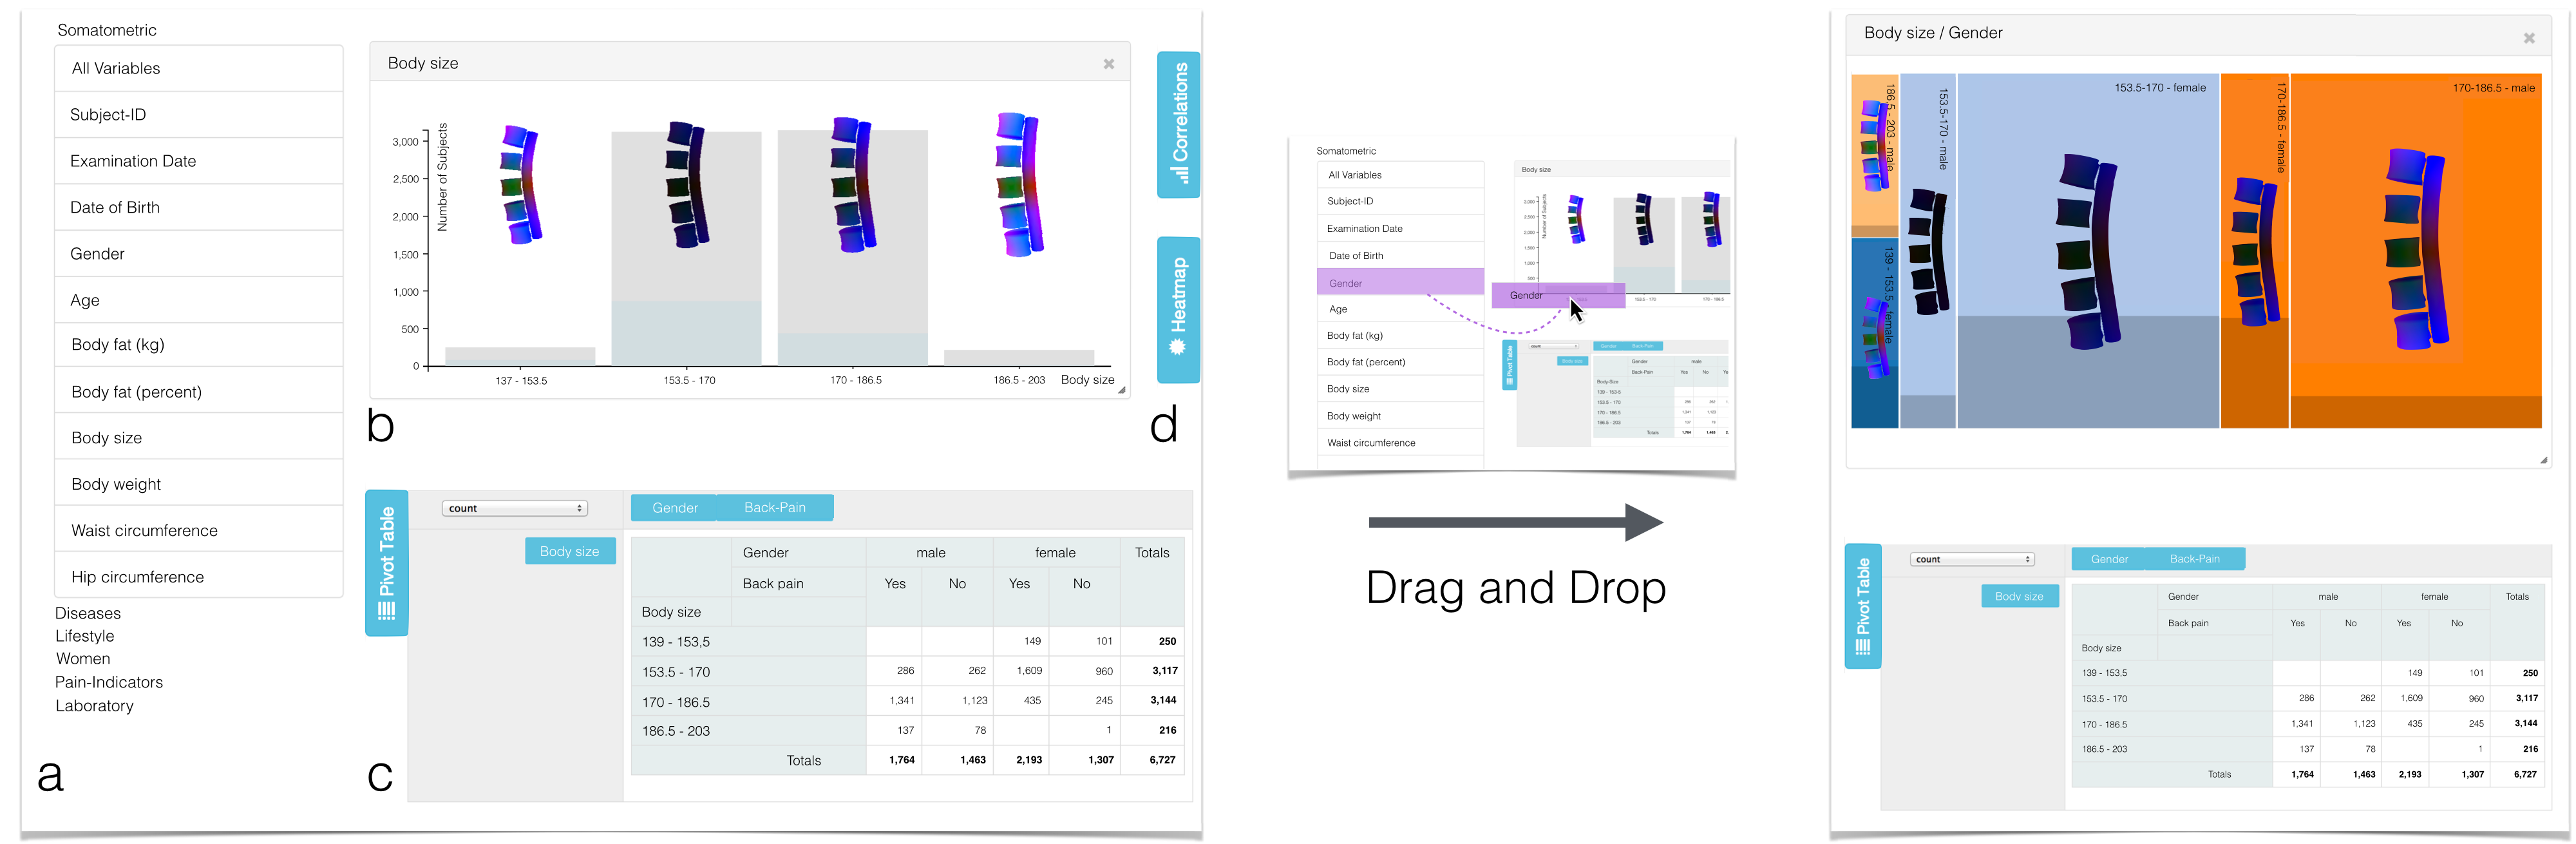
\includegraphics[width=1\textwidth, resolution=300]{figures/visualization}
 \caption{
 %
 (Left) Screenshot from the front-end, which is divided as follows: (a) The sidebar containing all features as well as the groups defined in the analysis process; (b) the canvas area where features can be added via drag and drop and the visualization is chosen automatically according to the data type; (c) the interactive pivot table showing the exact numbers for each displayed feature combination; \add{(d) Buttons to open panes containing the contingency matrix, contingency pane and pivot table}.
 %
 The data displayed is used to analyze the lumbar spine. Features can be added freely on the canvas via drag and drop.
 %
 Dropping the \emph{gender} parameter on the already plotted \emph{body size} container creates a mosaic plot combining both features (right).
 %
 \add{In a prior step, the user selected all subjects with diagnosed thyroid disorder.
 %
 These subjects are shown as shade in the visualization, denoting their share.
 %Their shares are denoted in the bar chart as blue and the mosaic plot as dark shade.
 %
 Subjects between 153.5--170~cm body size are more affected by thyroid disorder (box plot) and are mostly female (mosaic plot).}
 %
 \add{Distance to the mean mesh of subjects with thyroid disorder is encoded as red for x axis, blue to y axis and green to z axis.}
 %The lumbar spine models encode distance to the mean model using  \emph{color} 
 }
 \label{fig:visualization}
\end{figure*}
%-------------------------------- /Figure -------------------------------
Our proposed \emph{IVA} workflow consists of three major steps as illustrated in Figure~\ref{fig:InteractionLoop}: Feature selection, visualization and brushing.
%
A hypothesis-driven analysis usually starts with the selection of features, or shape groups derived from a shape-based clustering.
%
\add{Hypothesis generation with focus on image data starts with a shape-based clustering or an \emph{overview visualization} of all features.}
%
The feature is mapped using an automatically chosen visualization appropriate for its data type (described in detail in the following section).
%
The visualization techniques have to combine both image- and non-image data to set domain and range data in relation to each other.
%
In our system, the visualization can either be brushed or new features can be added to the analysis. 
%
%Brushing methods are subdivided using the previously described \emph{IVA} patterns.
%
Brushed regions are treated like categorical features, as they divide the subject space in the same way.
%
Selecting features also triggers a \emph{multivariate analysis} using contingency values (described in the following section) to highlight \add{associated} features.  %\rem{with selected features.}
%
A sample workflow using interaction and visualization techniques described in the next section can be seen in Figure~\ref{fig:visualization}.

% \subsection{Interaction and Visualization Techniques} \label{Interaction- and Visualization Techniques}
\section{System Design and Implementation} \label{Interaction- and Visualization Techniques}
%
The suitability of an interaction and visualization technique for epidemiological data depends on its ability to compare multiple data features at once while highlighting new associations.
%
The methods have to reflect the routines that epidemiologists take in order to be incorporated into their research.
%
Visual evaluations of data are therefore as important as methods allowing for numerical data analysis.
%
In the following sections we present the different parts of our proposed \emph{IVA} system for image-based cohort study analysis.
% \subsection{System Structure and Design} \label{Structure and Workflow}
\subsection{Design and Visualization Techniques} \label{Structure and Workflow}
% \begin{itemize}
% 	\item [x] Was sind die requirements des tools?
% 	\item [x] how it was decided to create this particular design
% 	\item [x] which kind of User interaction was made?
% 	\item [x] Spezielle Anforderungen durch Webseitenformat, weggehen von allgemeinen UI Elementen wie Menubar, keine Rechtsklickmenüs.
% 	\item [x] Entschieden eine saubere UI zu bauen, Unterscheide durch Whitespace akzentuieren. Interface in Fig. 3 zu sehen.
% 	\item [x] Wie wird interagiert, wie wird gebrusht, was wird gelinkt?
% 	\item [x] wie wird das Clustering initialisiert?
% 	\item auf Kontingenzmatrix mit verweisen als Teil des Interfaces (dieses auch noch anpassen)
% \end{itemize}
%Early it became clear that we have to rely a lot on online communication with our clinical partners due to their busy schedule and our large spatial distance towards each other.
\add{Early it became clear that we have to rely a lot on online communication due to the busy schedule and our large spatial distance towards each other.}
%
Hence we build our system using modern web technologies, described in detail in Section~\ref{implementation}.
%
By running the prototypes on server machines, software exchange became as easy as sharing a website link, giving us the opportunity to include the clinical experts easily in the development process.
%
Incorporating the \emph{IVA} workflow for image-centric cohort study data requires \emph{overview visualizations} as well as \emph{multivariate visualizations}, which bring image-derived information in context to non-image features.

The focus on web technologies is not without tradeoffs.
%
Classical UI elements, such as the menu bar or custom right click menus, are technically possible, but not common in this domain.
%
In favor of a clean layout, we designed the system without such components.
%
Since the previously described \emph{IVA} workflow allows for many different ways to analyze the data, we tried to make the interface as minimalistic as possible, treating the resulting space as \emph{canvas} for the data.
%
% \subsubsection{System Structure}
We divide the workspace into four major parts, as illustrated in Figure~\ref{fig:visualization} and \ref{fig:similarity}.
\begin{itemize}
		\item The \emph{sidebar}, which contains all epidemiological features. As cluster results group features like categorical features and are part of the sidebar as well (\add{Fig.~\ref{fig:visualization} (a)}).
	%
	\item The \emph{canvas} holding all visualizations. Elements can be added, arranged, resized and removed freely (\add{Fig.~\ref{fig:visualization} (b))}.
	%
	\item The interactive \emph{pivot table} gives detailed numerical information of the features in the canvas view. This view on the data is familiar to epidemiologists (\add{Fig.~\ref{fig:visualization} (c)}).
	%
	\item The \emph{contingency view} depicts relations for features in the canvas in an adjacency matrix (\add{Fig.~\ref{fig:similarity}}) and a \emph{contingency list}.
\end{itemize}

\paragraph{System Layout.}
We experimented with several layouts.
%
The initial idea was to make all components freely arrange- and resizable on a large \emph{canvas} area.
%
This idea was soon dropped since domain experts reported a cluttered workspace, which required a lot of scrolling.
%
The introduction of separate panes for the adjacency matrix, pivot table and sidebar, displayed with a mouse click on the corresponding button and sliding on top of the \emph{canvas} was considered more feasible (Figure~\ref{fig:visualization} shows the system with reeled-out pivot table pane).
%
All user-generated visualizations follow are part of the \emph{canvas} and can be arranged freely.
% are the  was to keep the concept of free arrangement for user-added 
%The resulting system can be seen in Figure~\ref{fig:visualization} (left).

\paragraph{Sidebar.}
The \emph{sidebar} is the only visible element when the system is opened (Fig.~\ref{fig:application} (a)).
%
It categorizes all features into different types, such as somatometric (measurements of the human body dimensions), disease- or lifestyle-related, pain indicators and laboratory data.
%
It also contains subject groups defined by automated shape clustering.
%
Groups are treated like features since they act the same by dividing the subject space into labeled categories.
%
Variables can be dragged from the sidebar into the canvas area for a \emph{feature localization}, which works as follows.
%
%This triggers an adaptive feature visualization suitable for the current data type.
%Bar charts show the distribution of manifestations of each variable in the sidebar.

\paragraph{Adaptive Feature Visualization.} \label{sec:AdaptiveFeatureVisualization}
\begin{figure}[htb]
 \centering
 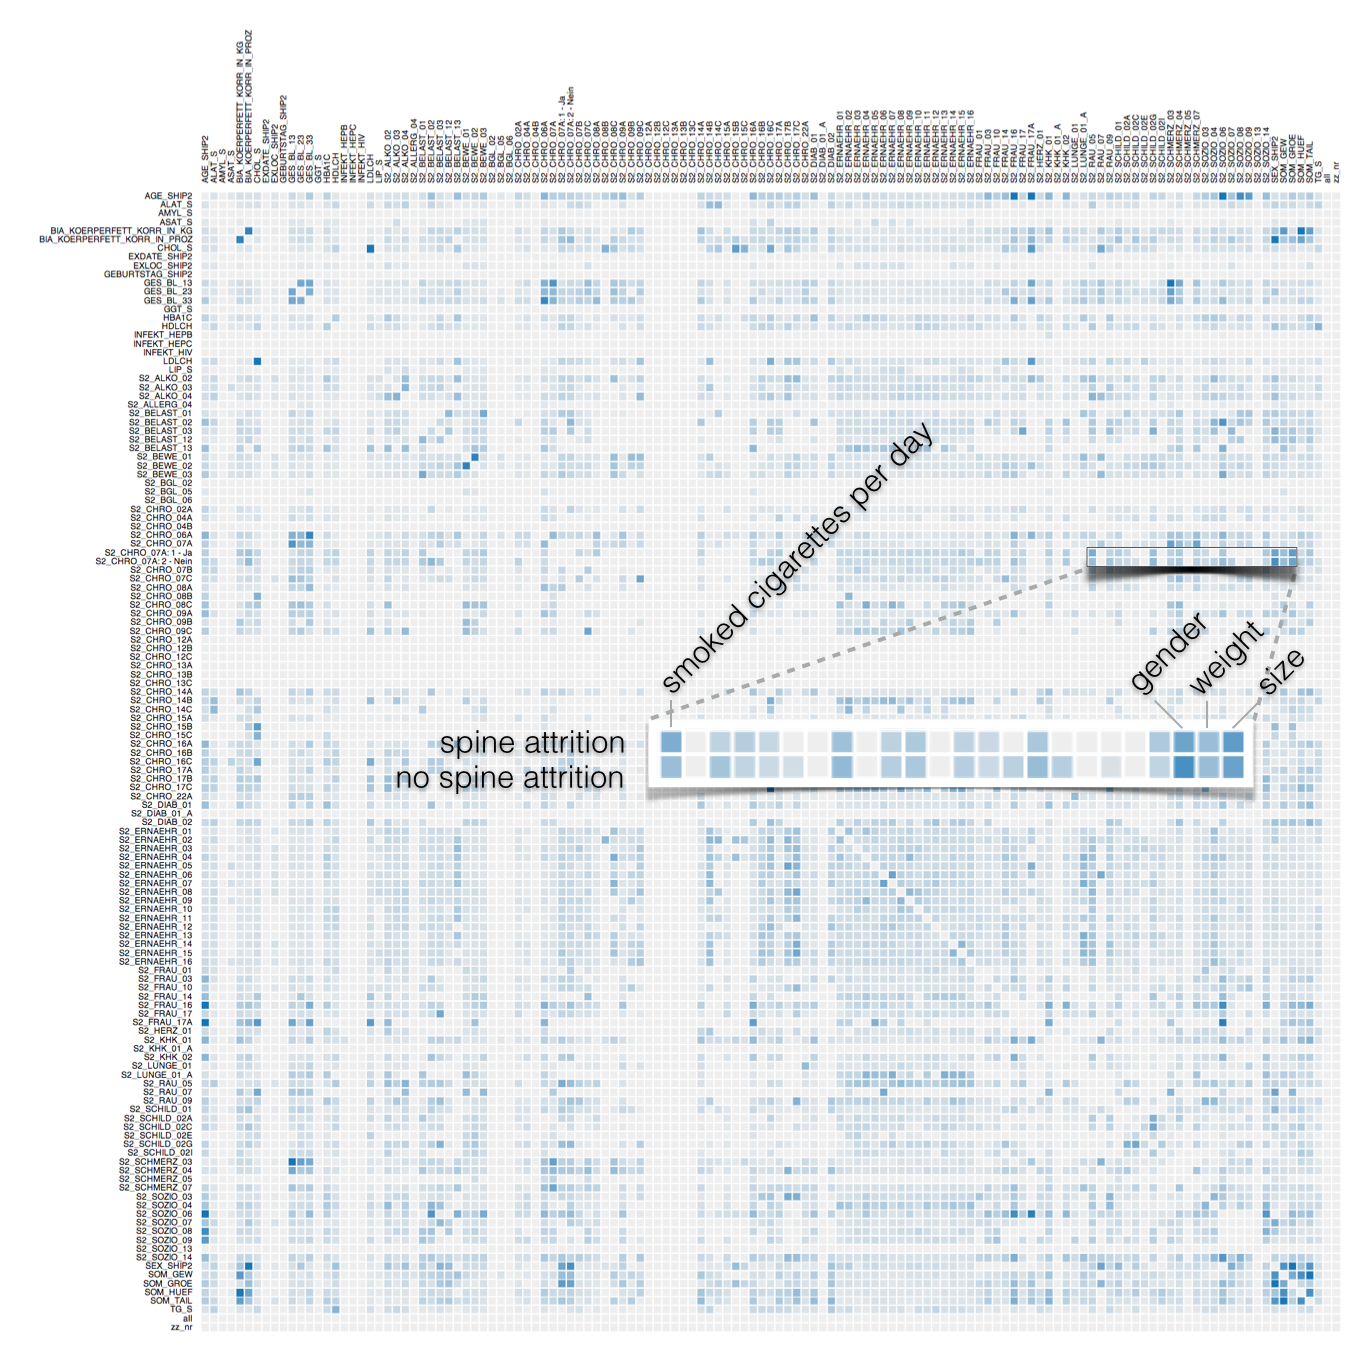
\includegraphics[width=3.5in]{figures/similarity_matrix}
 \caption{Adjacency matrix of 129 features (127 data set variables, 2 cluster results) with a grand total of 16,641 combinations.
 %
 Similarity is calculated using the \emph{Cram\'{e}r's V} contingency value.
 %
 Color brightness encodes association strength.
 %Mouse-over focuses a entry and highlights the feature names for better readability.
 Mouse-over an entry enlarges the feature names for better readability.
 %
 The enlarged excerpt shows associations for shape clusters of subjects with and without diagnosed spine attrition, which show associations between gender, weight, body height and smoking behavior.
 }
 \label{fig:similarity}
\end{figure}
The visualization type, inspired by \texttt{GPLOMS} \cite{GPLOMS, Francois2013}, is dynamically chosen based on the feature types and number to allow for \emph{multivariate analysis}.
%
Categorical data are either mapped to bar charts (single features) or mosaic plots (multiple features).
%
Figure \ref{fig:visualization} describes this dynamic adjustment.
%
Continuous data can be visualized using scatterplots (two features) or parallel coordinates (multiple features), but in epidemiology, this data type is usually categorized into ordinal groups of \emph{equal size}.
%
Since the number of categories often depends on the hypothesis, the discretization steps can be adapted dynamically.
%
Too many groups potentially generate sparse bins not suited for statistical evaluation.
%
Not enough groups overgeneralize information.
%
Adaptive discretization is an option, but imposes possible overfitting to the data.
%
Conclusions based on statistical relationships derived from groups already biased by feature distribution are heavily influenced by the used discretization.
%
Therefore we follow the convention to use bins of equal size.

%
%
Following Tufte's concept of \emph{small multiples} \cite{Tufte1983}, information derived from the medical image data are directly incorporated into the plot by including color-coded mean shapes for each manifestation (Figure~\ref{fig:visualization} (b)).
%
The 3D plots can be navigated using standard mouse input, the camera is synchronized between all views to enable direct comparison.
%
The distance from a group mean shape is mapped to the global mean using color.
%
This allows to assess local shape changes (Fig.~\ref{fig:visualization}) and is an important information to the epidemiologist.
%
Until now they were not able rapidly validate shape differences based on non-image features.
%
Dropping a feature on an existing plot adapts the visualization dynamically to allow for comparison (Fig.~\ref{fig:visualization} (right)).
% --- PARAGRAPH ---

To support \emph{feature localization}, subject groups can be brushed via a double-click on its representative in the visualizations.
%
Holding down the shift key allows to select multiple manifestations.
%
Brushed groups act as reference for the shape-visualization, calculating distances based on the mean-shape of the brushed selection.
%
%This allows to highlight distances between subjects
The share of subjects of this subgroup is linked to all other views (Fig.~\ref{fig:visualization} (left)).
%
If the user selects all female subjects in a visualization of gender distribution, all other displayed meshes are color-coded with their distance to the female mean and the share of female subjects is highlighted in the information visualization.
%Elements can be brushed using 
%Each plot can be brushed using widgets.
%
%Brush selections are propagated to all visualizations allowing for fast feature querying.

\paragraph{Pivot Tables.}
%Pivot tables are frequently used to present the data in epidemiological publications.
%
Epidemiologists are used to perform \emph{multivariate analysis} of groups based on table representations.
%
Thus, we decided to introduce an interactive pivot table.
%
These tables clearly convey the subject count in each group (see Figure~\ref{fig:visualization} (c)).
%
However, they quickly get confusing when they are divided into many subgroups.
%
We tackled this problem by making the order and number of displayed variables adaptable.
%
This also applies to the assignment of row or column variables.
%
Another way to avoid clutter is the user-driven selection of displayed variables.
%
To allow better comparison with respect to features, the values of each cell can also be displayed as percentage of the feature represented of either the row or column.
% TODO IMPLEMENT

\paragraph{Automated Feature Suggestion using a Contingency Matrix.}
%\rem{As previously discussed}
Highlighting potentially interesting values in the data set is one major benefits of the \emph{IVA}-powered approach and belongs to the \emph{multivariate analysis} pattern,  analyzing features outside the shape space.
%
Turkay et al. \cite{Turkay2013} used the approach to calculate key figures based on the distribution functions of each feature derived from the image data.
%
Since the majority of our data are categorical features, we have to employ different solutions.
%
The \emph{Cram\'{e}r's V} contingency coefficient can be used to calculate coherences between categorical variables \cite{CramerV}.
%
It is based on \emph{Pearson's $X^2$} distribution test \cite{ChiSquare}, which uses contingency tables holding the counts of subjects for all possible manifestations of two variables.
%
\emph{Cram\'{e}r's V} is defined as:
\begin{equation}
V = \sqrt{\frac{X^2}{N(k-1)}},
\end{equation}
where $X^2$ equals \emph{Pearson's chi squared}, $N$ is the total number of observations and $k$ is either the row or column count, depending on which one is lower.
%
$V$ yields values between $0$, meaning that two variables are completely independent, and $1$ indicating they are the same.
%
%Since \emph{Cram\'{e}r's V} is always positive, 
\emph{Cram\'{e}r's V} does not allow to infer about dependency direction.
%

It shares the same restrictions as \emph{Pearson's $X^2$}.
%
The expected counts in the contingency table have to be larger than 5 for $80\%$ of the entries and no expected value must be smaller than one \cite{Cochran1952}.
%
Some manifestations and feature combinations, which are only exposed by small subject groups, cannot be assessed with this technique.
%
They cannot be included into the epidemiological analysis, since statistical validation needs a minimum count to be valid.
%
The contingency matrix highlights correlations between all features. %of visualized features with features in the data set.
%
This aims to highlight features possibly associated with the focused hypothesis as well as trigger new hypotheses.
%
Contingency is visualized using an interactive adjacency matrix with association power mapped to color brightness.
%
The distinction whether an association is a confounder or an effect, depends on the context defined by the hypothesis and is a decision to be made by the domain expert.
%
The contingency matrix visualization is an \emph{overview visualization}, something the epidemiological community lacks and is in great need of.

\paragraph{Contingency Pane.}
Dropping a feature into the canvas area adds an entry for each manifestation of it to the \emph{contingency matrix}.
%
Testing sessions revealed that it was tedious to open the matrix every time a new feature is added. 
%A simple list of features, which correlate with the last added feature.
%
As a consequence, the \emph{contingency pane}, a table containing correlating features for the last added visualizations in descending order of the \emph{Cram\'{e}r's V} value was added.
%
\emph{Contingency pane} entries can be dragged and dropped into the \emph{canvas area} just like features in the \emph{sidebar}.
% Build after user request
%
\paragraph{Initialization and Clustering.}
Using feature suggestion allows to initialize the system with a set of potentially interesting visualizations.
%
After testing and domain expert feedback we dropped this idea.
%
Reasons for this are twofold.
%
Very often are high correlations obvious, such as gender with menstrual status.
%
Also, we observed that the variables of interest are dependent on the specialization of the domain expert (explained in detail in Section~\ref{application}).
% --- PARAGRAPH ---

Subject clustering is triggered automatically as \emph{local investigation} for each feature after it was added to the canvas by the user.
%
A status indicator at the bottom of the screen keeps the user informed about the pending clustering result, since the process can take up to ten seconds.
%
Clustering result are listed in their own category in the \emph{sidbar}.
%Since a clustering process can take up to ten seconds, a status indicator at the bottom of the screen keeps the user informed.
%
%\com{Clustering also automatically triggered}

% TODO: This can be an Section of it's own? Or part of the design?
\subsection{Implementation} \label{implementation}
\begin{figure}[htb]
 \centering
 \label{fig:technologies}
 %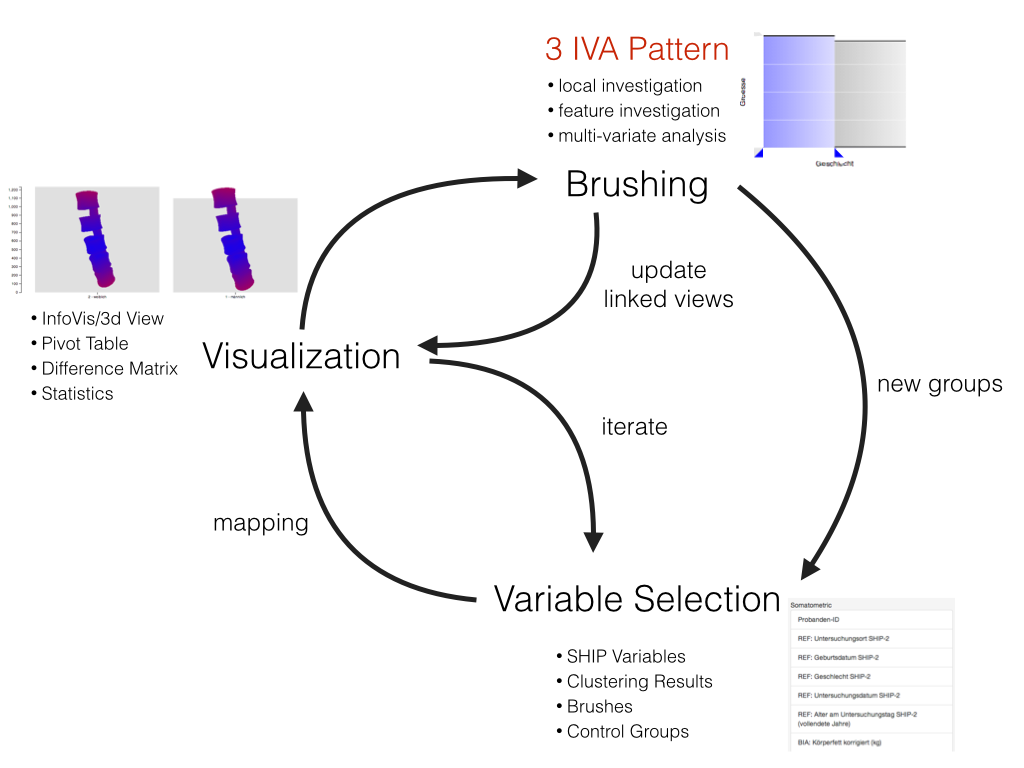
\includegraphics[width=1.5in]{figures/InteractionLoop}
 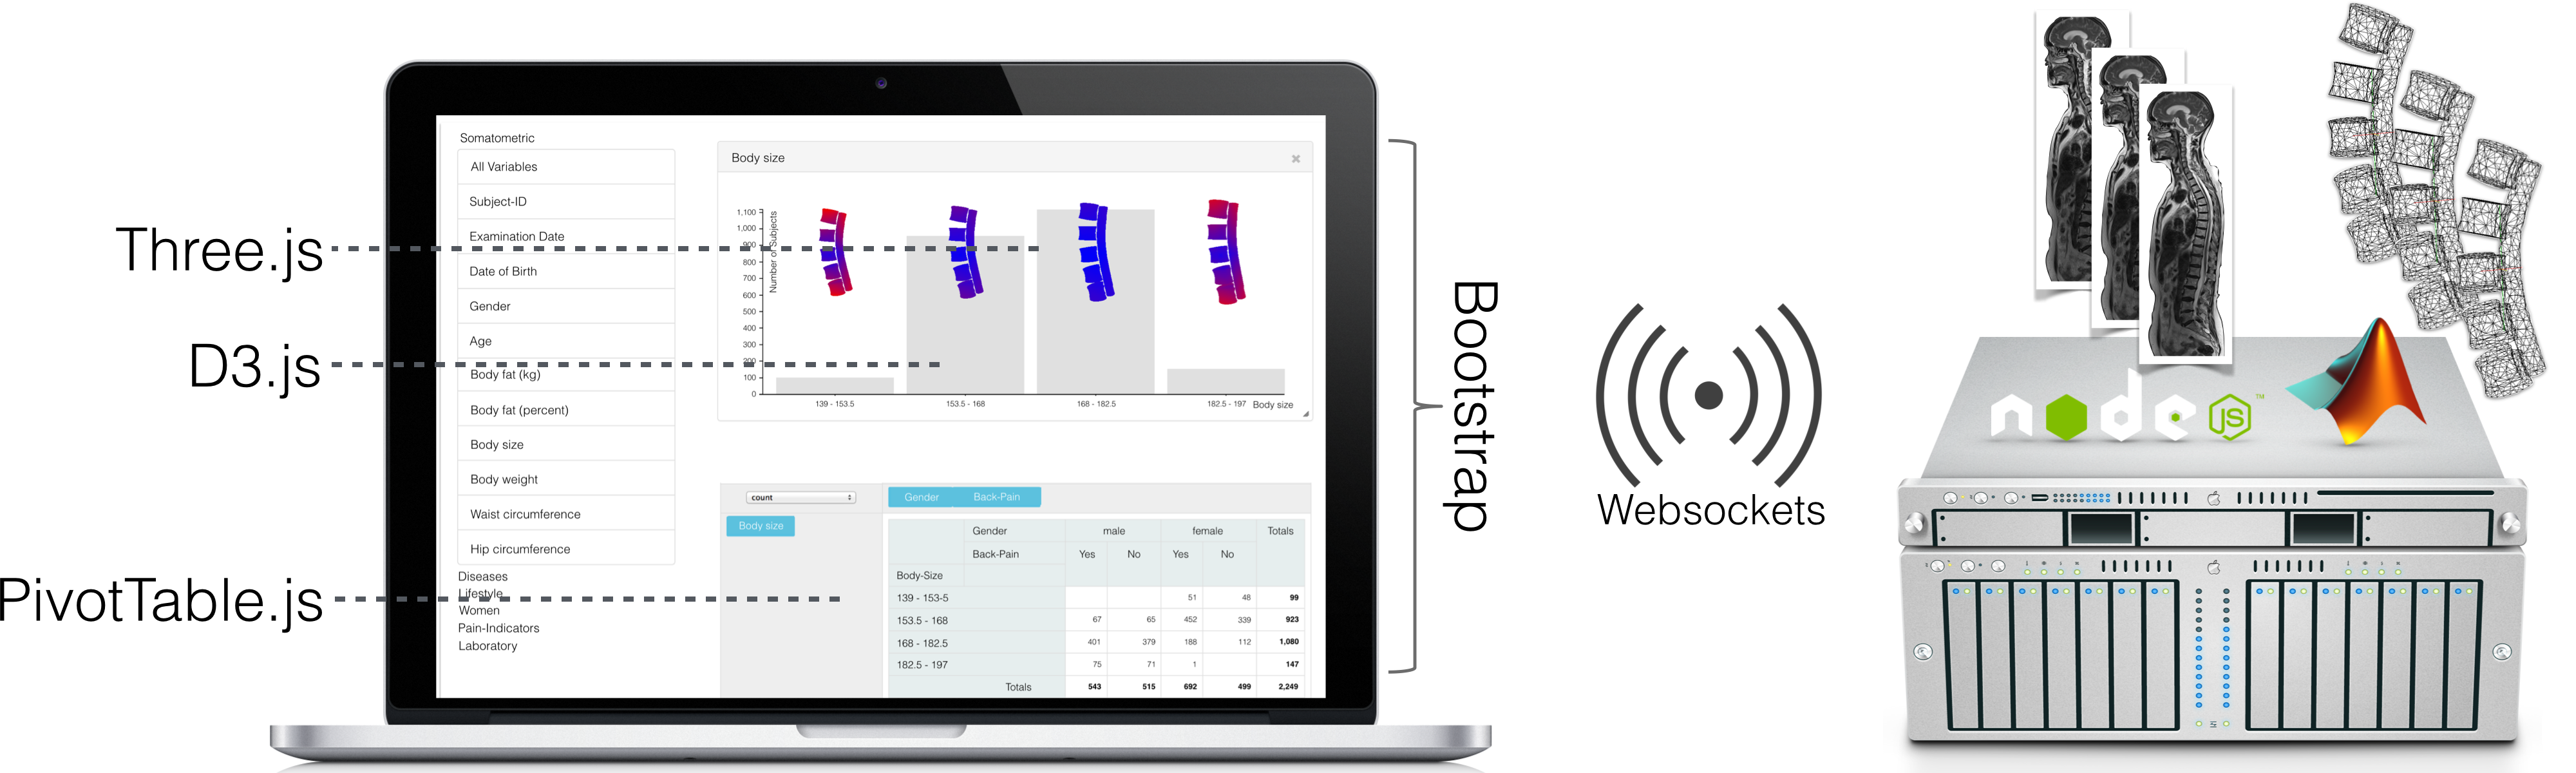
\includegraphics[width=3.5in]{figures/technologies}
 \caption{The front-end solution (left) uses \emph{HTML5}/\emph{CSS3}, \emph{WebGL} and \emph{SVG} to display the data.
 % 
 The \emph{NodeJS} based back-end (right) stores all image and non-image data and transfers it to connected clients.
 %
 All computation-heavy operations, such as calculation of mean shapes or distances, are performed on the server-side. 
 %All computation-heavy operations, such as calculation of mean shapes or distances, as well as statistical processing are done by the server to keep hardware requirements of client systems low. 
 %
 Client-server communication is accomplished via the \emph{Websocket} protocol.
 }
\end{figure}
In this section we discuss how we implemented the presented methods using open web standards.
%
To provide a fast communication loop between method development and expert input, we decided to rely on modern web technologies.
%
In addition to the obvious advantages of web technologies, the following aspects are crucial for our work:
\begin{itemize}
%	\item No additional software needs to be installed, most people use a decent state-of-the-art web browser, even on mobile devices.
	\item The client-server structure allows for employing heavy computation on a server machine and transferring results to the client.
	\item \add{Disk-space demanding image data remains on the server and elements can be transferred on demand.}
	%\item Since image data for thousands of subjects requires hundreds of gigabytes disk space, it can remain safely on the server and elements can be transferred on demand.
	%
	High confidentiality standards of the data are met by \add{password protecting the access.}%restricting access via an account system.
	\item Recent developments in \emph{WebGL} applications running in browsers with near-native performance result in many open source libraries, which are well documented and driven by active communities. We use \emph{WebGL} for rendering shape information.
%	\item Web technologies are free.
\end{itemize}
These advantages do not come without drawbacks.
%
Sophisticated libraries/languages, such as the \texttt{Visualization Toolkit} (\texttt{VTK})\footnote{Developed by Kitware Inc; \href{http://vtk.org}{\texttt{vtk.org}}} or \texttt{R}\footnote{Open Source; \href{http://r-project.org}{\texttt{r-project.org}}} for statistics, are either not available at all or only accessible through complex client-server systems.
%
Therefore, many standard methods had to be written from scratch.
%
%\rem{The user needs a fully updated modern web browser, which supports these new technologies, such as WebGL.}
%Due to missing ports of sophisticated and specialized libraries/languages, such as the \texttt{Visualization Toolkit} (\texttt{VTK})\footnote{Developed by Kitware Inc; \href{http://vtk.org}{\texttt{vtk.org}}} or \texttt{R}\footnote{Open Source; \href{http://r-project.{\texttt{r-project}}org}} for statistics, many standard methods need to be written from scratch.
%Due to missing ports of sophisticated and specialized libraries/languages, such as the \texttt{Visualization Toolkit} (\texttt{VTK})\footnote{Developed by Kitware Inc; \href{http://vtk.org}{\texttt{vtk.org}}} or \texttt{R}\footnote{Open Source; \href{http://r-project.{\texttt{r-project}}org}} for statistics, many standard methods need to be written from scratch.
%

The back-end is written using \texttt{NodeJS}\footnote{Developed by Joyent Inc, \href{http://nodejs.org}{\texttt{nodejs.org}}}, which is based on the Google V8 Javascript runtime environment.
%
Due to its event-driven non-blocking I/O model it is fast and does not freeze in case of heavy workload such as mesh processing.
\\\\
Non-image data for all subjects including the data dictionary is stored in a JSON file on the server.
%
Image data are available as raw DICOM files.
%
Segmentation masks of anatomical structures are represented as meshes, suited for comparing subjects.
%
The requested data are transmitted when a client connects.
%
The server performs heavy statistical tasks, such as calculation of \emph{Cram\'{e}r's V} values for all feature combinations in order to keep the computation time on the client as low as possible.
%

The front-end is created using \texttt{Bootstrap}\footnote{Developed by Twitter, \href{http://getbootstrap.com}{\texttt{getbootstrap.com}}} as foundation for the layout and basic UI elements using \texttt{HTML5}, \texttt{CSS3} and \texttt{Javascript}.
%
Information visualizations such as scatterplots and bar charts are created using the popular \texttt{Data-Driven Documents (D3.js)} library \cite{D3}, which works well for attaching data to visible elements like vector graphics and provides powerful transformation and mapping tools.
%
The pivot table implementation was adapted using \texttt{PivotTable.js}\footnote{Developed by N. Kruchten, \href{http://nicolas.kruchten.com/pivottable}{\texttt{nicolas.kruchten.com/pivottable}}}.
%
\texttt{Three.js}\footnote{Originally developed by R. Cabello, \href{http://threejs.org}{\texttt{threejs.org}}} allows GPU-accelerated data rendering using \texttt{WebGL}.
%
Communication between client and server is enabled via the WebSockets protocol.
%
Since our clustering algorithms are written in \texttt{MatLab}\footnote{Owned by The MathWorks, \href{http://mathworks.com}{\texttt{mathworks.com}}}, we had to access them using the \texttt{NodeJS} server.
%
We accomplished this by converting it to a parameterized standalone console application that is spawned by \texttt{NodeJS} on client request and then reads the result from the console standard out and returns it to the client.
%
All parameter-steered console applications can be incorporated in this context.
\\\\
\section{Application} \label{application}
This section describes how the presented \emph{IVA} workflow is used in the epidemiological application.
%
We conducted a qualitative evaluation with two domain experts on a data set compiled to analyze lower back pain. 
%
This is one of the most common reasons for an adult to see a physician in the Western civilization \cite{Backpain}.
%
Epidemiological analysis of lumbar back pain, such as the work of Harreby et al. \cite{Harreby1996}, is largely focused on non-image information.
%
In comparable studies, only a few shape-related features are included \cite{Lang2011}.
%
%To our knowledge, this is the first approach, where shape-related information of the whole lumbar spine is analyzed along with other epidemiological features.
%
Determining risk factors in this area can lead to particularly affected risk groups, prognostic features for diagnosis and treatment of lumbar back pain and a better understanding of effects of preventive measures, such as occupational health and safety regulations \cite{Fletcher2012}.
% Determining risk factors in this area can lead to \cite{Fletcher2012}
% \begin{itemize}
% 	\item a better understanding of effects of preventive measures, such as occupational health and safety regulations,
% 	\item prognostic features for diagnosis and treatment of lumbar back pain, and
% 	\item determination of particularly affected risk groups.
% \end{itemize}
%
Characterizing the healthy aging process of the spine is a long-term goal for determining age-normalized probabilities for spine-related diseases by incorporating individual risk factors.
%
\subsection{The Lumbar Spine Data Set}
%We divide the data set into image and non-image data.
%
\add{
There are 127 features describing diagnosed diseases, lifestyle factors, women-specific factors, pain indicators, laboratory values and somatometric features for 6.753 subjects (4.420 from \texttt{SHIP-Trend-0} and 2.333 from \texttt{SHIP-2}).
%
Since data acquisition protocols between these two cohorts are identical, the features between the two cohorts are comparable.
}
%
\add{The data contains 30 metric, 7 nominal, 29 ordinal and 62 dichotomous epidemiological features.
%
Somatometric features include measures of the human body, such as body height, weight and body fat percentage as well as gender.
%
These measures are reliable and complete.
%
Other features, such as pain indicators or lifestyle indicators (e.g. physical activity) are more subjective and less reliable.
%
There are also features missing for each subject, such as features building upon each other (e.g. Do you have high blood pressure? Which medication is prescribed against it?).
%
Therefore some manifestations are sparsely populated, which makes statistical evaluation challenging.
%
%Another challenge the 
}
%

The MRI data was acquired for each subject on a 1.5~Tesla scanner (Magnetom Avanto; Siemens Medical Solutions, Erlangen, Germany) by four trained technicians in a standardized way.
%
\add{The spine protocol consisted of a sagittal T1-weighted turbo-spin-echo sequence ($1.1\times1.1\times4.0~mm$ voxels) \cite{Hegenscheid2013}. %(676 / 12 [repetition time msec / echo time msec]; 150$^\circ$ flip angle; 500~mm field of view; $1.1\times1.1\times4.0~mm$ voxels) and a sagittal T2-weighted turbo-spin-echo sequence (3760 / 106 [repetition time msec / echo time msec]; 180$^\circ$ flip angle; 500~mm field of view; $1.1\times1.1\times4.0~mm$ voxels) \cite{Hegenscheid2013}.
}
%The spine protocol consisted of sagittal T1- and T2-weighted turbo-spin-echo sequences with rather large slice distance only sufficient for characterizing the lumbar spine \cite{Hegenscheid2013}.

\subsubsection{Data Preprocessing} \label{application:Data Preprocessing}
The data are preprocessed as described in Section~\ref{Data Preprocessing}.
%
\paragraph{Non-Image Data.} 

To ensure a fast and easy data access outside of statistical processors like \texttt{SPSS}, the data was exported to the JSON file format.
%
\add{
Since it lacks export methods for data dictionaries, we used \texttt{SPSS} to export our data to the 'SAS v9+' format, which saves the data labels, and exported the data values as non-labeled CSV.
%
A short script combined both data sources to a JSON file.
%
The data types had to be transferred manually.
}
%
\add{Each feature is stored as an object containing the data as array it's data type, a detailed description and data dictionary translating value or error IDs to values.}
% \begin{itemize}
% 	\item the data as array of values--categorical data and error codes are stored using IDs,
% 	\item the data type (continuous, nominal, ordinal, dichotomous),
% 	\item a detailed description of the feature, and
% 	\item the data dictionary translating value or error IDs to values.
% \end{itemize}
% Each feature is stored as an object containing:
% \begin{itemize}
% 	\item the data as array of values--categorical data and error codes are stored using IDs,
% 	\item the data type (continuous, nominal, ordinal, dichotomous),
% 	\item a detailed description of the feature, and
% 	\item the data dictionary translating value or error IDs to values.
% \end{itemize}
%
% Binning: https://www.researchgate.net/post/What_metric_best_captures_the_information_loss_when_binning_a_large_data-set_into_a_histogram_representation
Continuous variables are discretized to allow for \emph{Cram\'{e}r's V} contingency coefficient assessment.
%
We set the number of groups to five, to allow for contingency assessment.

\paragraph{Image Data.} \label{Image-Data}
The lumbar spine was detected in the image data using a hierarchical finite element method by Rak et al. \cite{Rak2013}.
%
This semi-automatic method requires the user to initialize the tetrahedron-based finite element models (FEM) with a click on the L3 vertebra.
%
Two user-defined landmarks on the top and bottom of the L3 vertebra are used to obtain an initial height estimation of the model.
%
It uses a weighted sum of T1- and T2-weighted MR images to detect the lumbar spine shape.
%
The registered models capture resilient information about the shape of the lumbar spine canal as well as the position of the L1-L5 vertebrae \cite{Klemm2013VMV}.
%
Due to incorrect initialization, strongly deformed spines, contrast differences and artifacts, the model was not able to detect lumbar spines for all subjects.
%
We obtained and worked with 2.540 tetrahedron models of the lumbar spine.
%
For clustering, we extracted the centerline of the lumbar spine canal, which captures information about lordosis and scoliosis (the medical terms for spine curvature \cite{Klemm2013VMV}).

%-------------------------------- Figure --------------------------------
\begin{figure*}[htb]
 \centering
 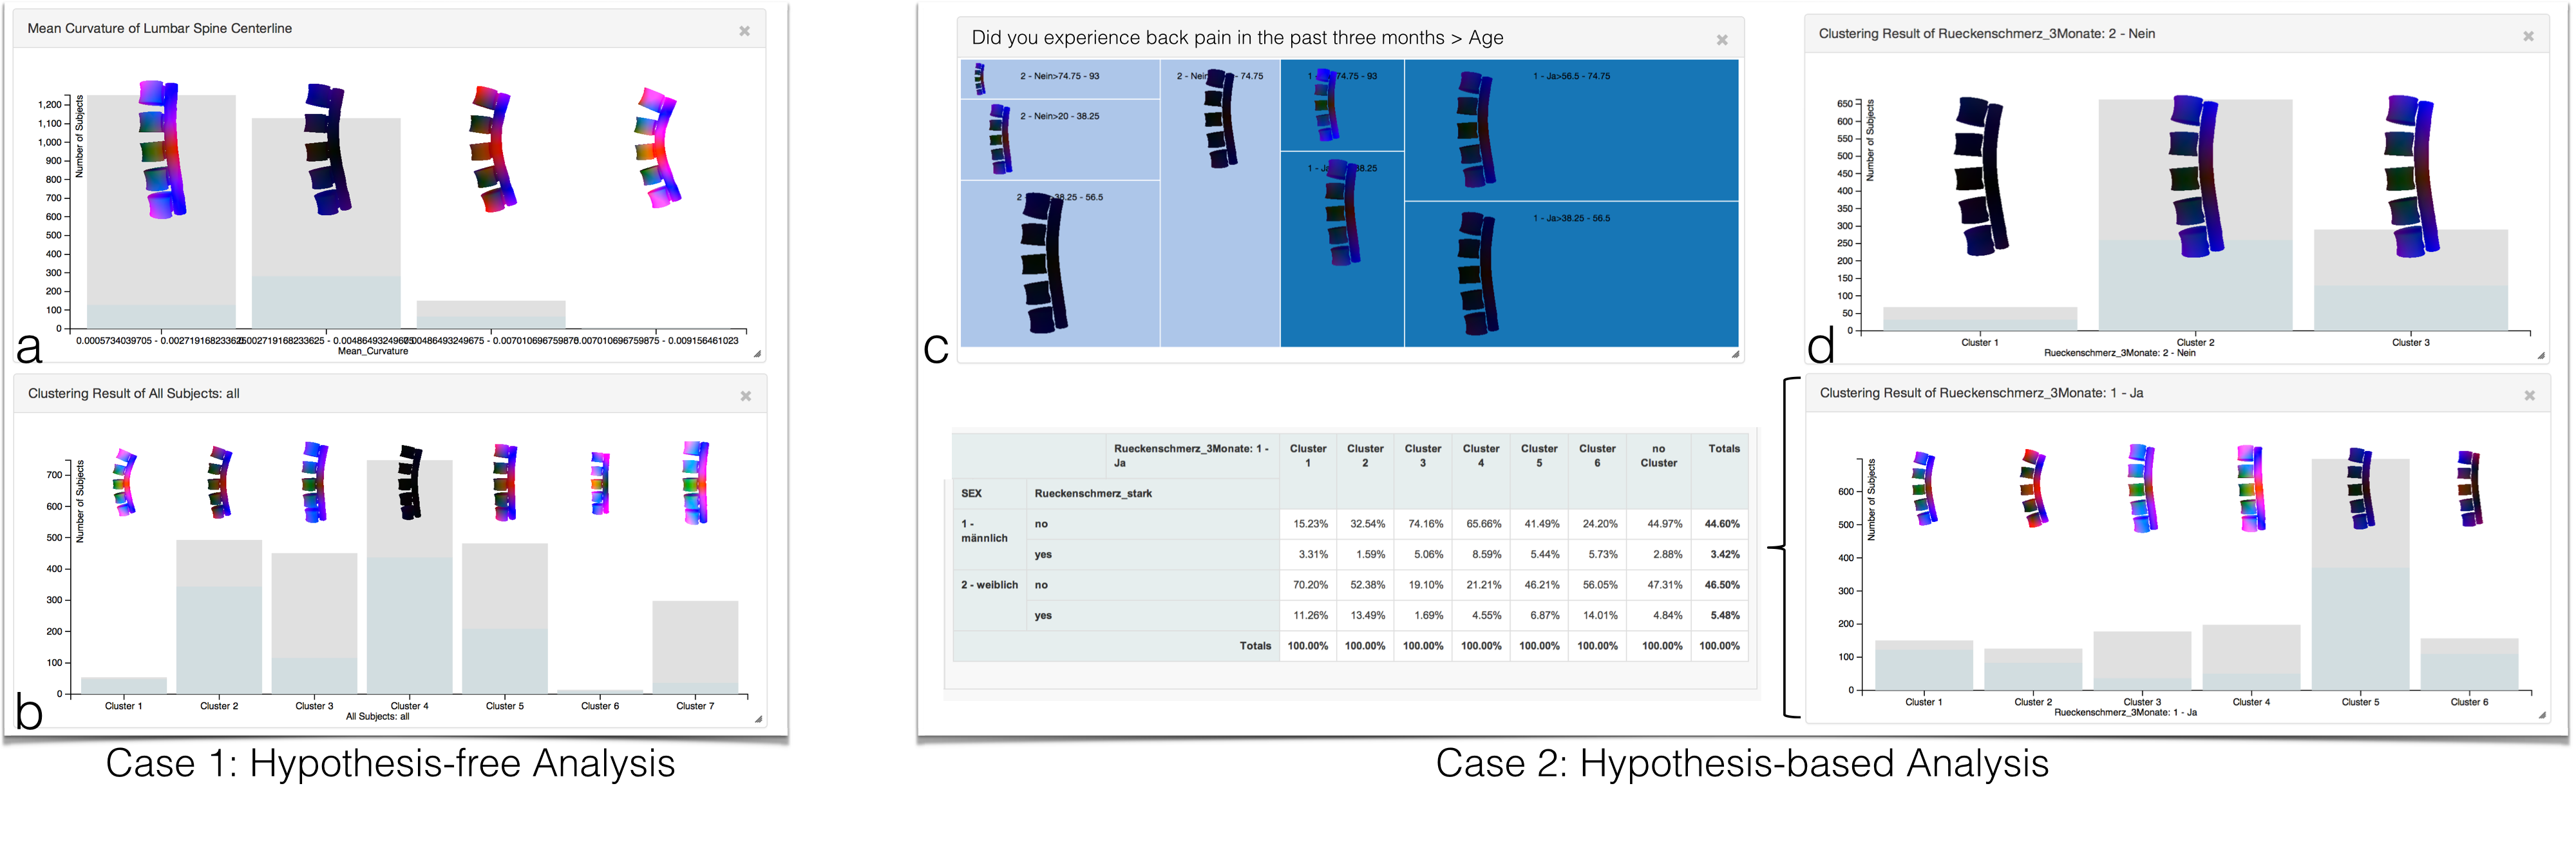
\includegraphics[width=1\textwidth, resolution=300]{figures/evaluation}
 \caption{Various case study results.
 %
 (a) Mean curvature of lumbar spine canal plotted against the mean shape of 58-74 years old female subjects (light-blue bars).
 %
 Note the high amount of this subject group relative to the total count in the third group compared. The last group only contains four outlier-subjects.
 %
 (b) Clustering of all subjects yields seven groups, where Cluster~4 assembles the mean. The light blue bars indicate the share of females in the group.
 %
 (c) A mosaic plot mapping age against dichotomous questionnaire answer to ``\emph{Did you experience back pain in the past three months?}''.
 (d) Clustering result of ``\emph{Did you experience back pain in the past three months?}'' Yes/no with female share in each group. 
 %
 Cluster 1 and 6 for answer ``\emph{Yes}'' contain mostly women.
 %
 The pivot table shows how many subjects with strong back pain are in each cluster for answer ``\emph{Yes}''.
 %
 Subjects in Cluster 1, 2 and 6 report strong back pain more often than subjects in other clusters.
%Female subjects are selected as reference for all plots, except for (c) The light blue selection in the bar charts represent the female share. }
 }
 \label{fig:application}
\end{figure*}
%-------------------------------- /Figure -------------------------------
\subsubsection{Shape Visualization and Clustering}
%
The tetrahedron-based detection model consists of corresponding grid points for each structure instance.
%
This allows to calculate shape distance and similarity.
%
This information is used to calculate mean shapes as described in Section~\ref{Interaction- and Visualization Techniques}.
%
Shape distance between to mean meshes is mapped to color (recall Fig.~\ref{fig:visualization}).
%
%For dichotomous variables, the color codes distances between mean shapes of the two groups, for variables with more than two manifestations it encodes the distance to the global mean shape of all subjects).
%

Shape-based clustering is carried out via agglomerative hierarchical clustering of the spine canal centerlines (recall Section~\ref{application:Data Preprocessing} and \cite{Klemm2013VMV}).
%
Since the ``correct'' number of clusters in a given group is unknown, an estimate is computed by means of the knee/elbow method \cite{Salvador2004}.
%
The method has proven to produce sound results on a preliminary data set and was able to reproduce textbook knowledge \cite{Klemm2013VMV}.
\subsection{Participants, Setup and Procedure}
%
%Lam et al. divide evaluations of Visual Analysis systems in two categories, 
%
%\com{Anmerkung von Steffen einbauen: Evaluierung geht um fachliches Feedback - Wissen über epidemiologie UND rücken und wissen um die Daten - deswegen schwer ganz viele Experten ranzuziehen}
Guided by the work of Lam et al \cite{Lam2012}, we conducted an investigation of \emph{Visual Data Analysis and Reasoning} (\emph{VDAR}).
%
This approach aims to characterize the systems ability to explore data, discover knowledge, generate hypotheses and help formulating decisions.
%
Since it is hard to quantify these outcomes, Lam et al. suggest case studies for the \emph{VDAR} by applying the think aloud protocol to understand the domain experts observations, inferences and conclusions when using the system.

Our participants are two epidemiological domain experts who also co-authored this publication.
%
HV and KH are practicing physicians with focus on epidemiological research.
%
HV is a specialist in internal medicine (23 years of experience) and also the head of the SHIP, KH a radiologist (9 years of experience) and responsible for the MRI data acquisition of the study. %and has a deep understanding on the available image data.
%
%(Their expertise and experience with the data in their day to day research make them aware of the problems associated with the analysis of medical cohort study data.)
%
\paragraph{Setup.} Due to the large geographical distance, the evaluation was done completely web-based.
%
%Our focus on web technologies right from the beginning made it easy to 
%Since one major reason for the focus on web technologies, no software needed to be exchanged.
%The experts accessed the prototype by simply entering the website link into their browser of choice, no exchange of software was required.
The experts accessed the prototype by entering the website link into their browser of choice, no exchange of software was required.
%Since our prototype ran on a local server, simply needed the homepage link to access the prototype.
%
%A website link was send to the users, which they could open with their browser of choice and start using the tool.
%
User input was observed using screen sharing.
%
Communication was enabled via webcam supported voice over ip.
%
The total setup time including installing the screen sharing application was about five minutes.
%
Video-recordings of the sessions allowed a detailed evaluation afterwards.%made a possible to evaluate the sessions later on.
%
\paragraph{Procedure.}
At first, we controlled mouse and keyboard of the participants PC and demonstrated the basic functionalities of the system.
%
%This included the contingency matrix, the correlation view, how to introduce feature visualizations, how the color coding of differences works and the pivot tables.
%
As they understood the concepts, we handed over the mouse and keyboard control and only observed from this point on.
%
The epidemiologists were given two tasks: one hypothesis-free analysis of the data and one starting with an assumption.
%
For each case we conducted one analysis with each expert.

% \subsection{Exploratory Analysis of the Lumbar Spine Data Set}
\subsection{Case 1: Hypothesis-free Analysis} \label{Hypothesis-free analysis}
Analyzing the data set without prior hypothesis requires a starting point giving an overview over the data \cite{Shneiderman1996}.
%
With our tool, there are two ways to achieve this.
%
Performing a \emph{local investigation} by clustering all subjects or use the contingency matrix for a \emph{multivariate analysis}.
%
The latter was chosen first by both experts.
% The latter was chosen first by the domain expert with radiological background.
%
%They pointed out the high potential they see in this visualization, because it allows to look at the data in an unbiased way.
%They pointed out the benefits of the possibility to look at all variables in the context of each other.
Before, they were not able to to look at all variables in the context of each other.
%
%
To cite one expert, the contingency matrix ``illumunates the data black box'', making it possible to look at the data unbiased from assumptions.

\paragraph{Analysis 1.}
%
The radiologist (KH) was looking for correlations with shape-related features in the data, finding that they correlate with \emph{leg pain}, \emph{age}, \emph{body height} and \emph{hormone replacement therapy status}.
%
Due to the dense mapping of information in the contingency matrix it was suggested to make this visualization full screen.
%Many correlations observed in this view 

After this initial overview, KH performed a \emph{multivariate analysis} by introducing features, such as \emph{age}, \emph{waist circumference}, \emph{weight} or \emph{lumbar spine canal curvature} as bar charts views into the canvas area and selected subgroups to see how they are distributed and if they could observe unusual behavior in the mean-shapes.
%
This pointed out problems with the used categorization method splitting numerical variables into equally-sized ordinal bins.
%
If a feature contains outliers, such as \emph{waist circumference} (e.g. by subjects with morbid obesity) this approach leads to sparse categories, making it hard to calculate associations.
%
The proposed expert solution for this is categorization using quantiles/quartiles and is described in detail in Section~\ref{Lessons Learned}.

A \emph{multivariate analysis} using the \emph{Cram\'{e}r's V} contingency values for subjects with strong lumbar spine curvature showed, that these subjects are primarily females between 58-74 years who also report pain radiating from their back into other body regions Figure~\ref{fig:application}(a).
%
%\com{Allgemein: Workflow noch einmal grob beschreiben - Overview first, details on demand}
%
\paragraph{Analysis 2.}
% \begin{figure}[htb]
%  \centering
%  %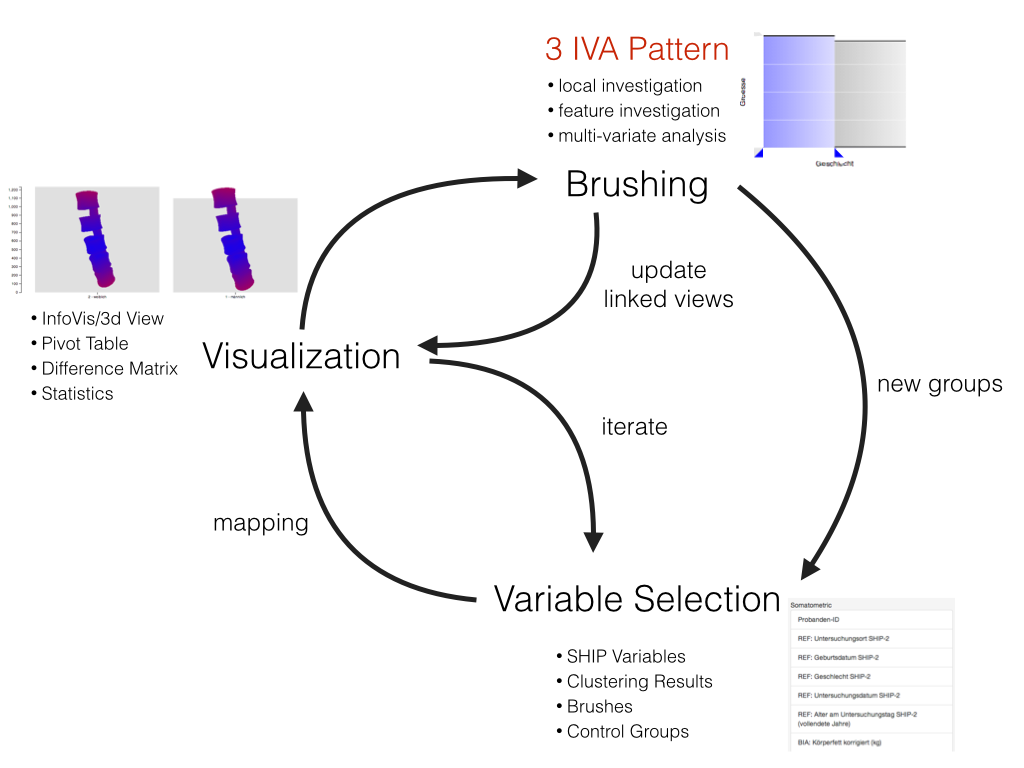
\includegraphics[width=1.5in]{figures/InteractionLoop}
%  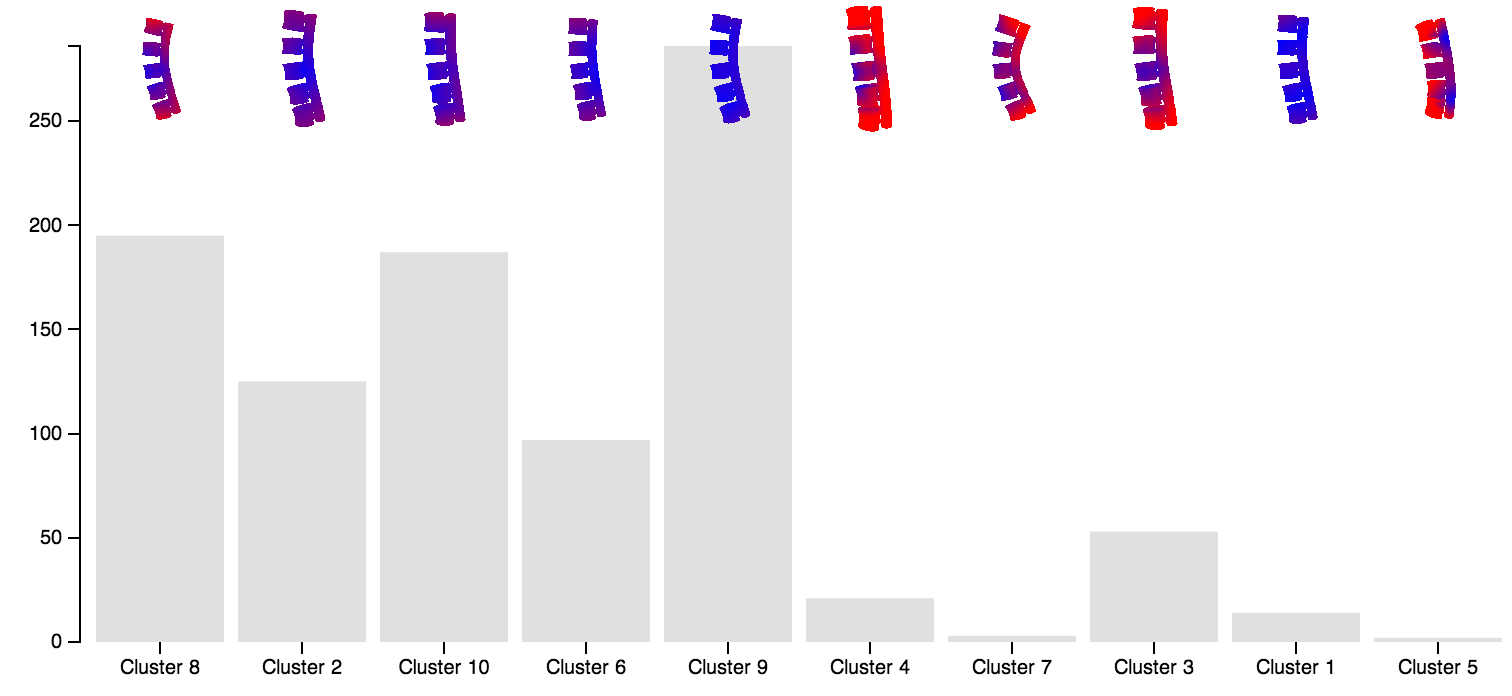
\includegraphics[width=3.5in]{figures/hypothesisfree}
%  \caption{(a) Clustering result of all subjects. The bar chart height indicates the number of subjects in the cluster. The difference to the mean shape is color-coded, whereas blue represents no difference and red a large difference. (b) A pivot table relates cluster results to gender and employment status. Cluster 8 is striking because of the high proportion of women, while cluster 2, 3, 4 contain almost only men.}
%  \label{fig:hypothesisfree}
% \end{figure}
%
HV started also with a \emph{multivariate analysis} using the contingency matrix to analyze non-image features, such as age-associated parameters like \emph{income}, \emph{blood fat values} or \emph{number of born children}, but found no associations of interest.
%
Therefore, he applied the \emph{local investigation} pattern by a shape grouping step using shape-based clustering via dragging the \emph{All subjects} from the sidebar into the canvas area, triggering the shape clustering.
%Shape-based hypothesis-free exploration starts with the \emph{local investigation} pattern by a shape grouping step using shape-based clustering.
%
The results for this step can be seen in Figure~\ref{fig:application} (b).

Cluster 4 represents subjects with average shape.
%
Other shapes differ with respect to size, such as cluster 2, 3, 7, where the last one and cluster 5 also represent a more straight spine, which is usual for subjects with larger body size.
%
Cluster 1 and 6 contain outliers, characterized by their unusual shape and small number.
%
%Cluster 8 has the second largest number of elements and was therefore of special interest.
%
%To perform an automatic feature suggestion using a \emph{multivariate analysis} by looking at \emph{Cram\'{e}r's V} contingency values of in the contingency pane.
To get an overview over the suggested features, the user opened the contingency pane to perform a \emph{multivariate analysis} by looking at \emph{Cram\'{e}r's V} contingency values of all clusters, revealing a strong correlation with \emph{gender} and \emph{body size}.
%
Therefore another \emph{multivariate analysis} was carried out by the feature \emph{gender} to the canvas from the contingency pane and selecting all female subjects (Fig.~\ref{fig:application} (b)).
%
Cluster 1 contained primarily female subjects.
%
Contingency values for this cluster revealed correlations with \emph{leg fatigue}, \emph{physically heavy work}, \emph{body weight}, \emph{dyspnoea} and \emph{headache intensity}.
%
%This revealed associations of this group with employment status, gender, body size, age, thyroid nodules and blood fat value.
%
Since it is a pain indicator, headache was of special interest and was further investigated by incorporating a pivot table setting \emph{headache intensity} in relation to cluster affiliation.
%
It was found, that cluster~1 subjects report heavy headaches more frequently than other subjects.
%Another \emph{multivariate analysis} using a pivot table set gender and employment status in relation to clustering affiliation\add{.} 
%
%\add{It s}hows that cluster~8 contains mostly women and also has a larger unemployment rate (see Figure~\ref{fig:hypothesisfree}), while the overall employment rate of women and men in the data set is almost exactly 50\%.
%
%While all observed features seem to be plausible associations related to back pain, the values indicate that cluster~8 contains subjects with chronic back pain radiating to the legs.
%
%Metabolic parameters, such as blood fat and blood sugar, are also possibly associated features.
%
%The employment status is a feature relating to many different lifestyle factors such as income or nutrition as well as age and might act as confounder.
\\\\
The experts emphasized the importance of methods providing an overview over the data for hypothesis generation.
%
With the presented \emph{IVA} approaches they were quickly able to confirm medical knowledge as well as elaborate new hypothesis.
%
We observed, that the domain experts are more likely interested in features they are familiar with and have personal clinical experience with.
% TODO: Contingency Matrix or Adjecency Matrix
%\com{00.44 Clustering-Ergebnis Weiblich und Arbeitspensum Alter}

\subsection{Case 2: Hypothesis-based Analysis}
If the user proposes a hypothesis about a relation between a non-image feature regarding shape, the workflow slightly differs from the hypothesis-free analysis.
%
The starting point follows the \emph{feature investigation} pattern, where a feature of interest is selected by dragging it into the canvas area and viewing the subject's distribution as well as their shape differences.
% \paragraph{Analysis 1.}
% The radiologist performed a \emph{feature investigation} by dragging the age variable into the canvas area, observing that age-bins 36-52 years and 52-68 years are nearly identical to the global mean, while 20-36 years and 68-84 years differ in size.
% %
% Performing a \emph{multivariate analysis} by selecting only female subjects via the additionally added gender feature it was observed, that distance was closest to subjects of 68-84 years old and largest to 20-36 years old.
% %
% The expert argued that this is most likely due to the shrinking of the spine with increasing age, making it more similar to the female average spine which is smaller than the global average \com{(00.29)}.
% %
% 
\paragraph{Analysis 1.}
Hypothesis: ``\emph{Back pain is associated with age and lumbar spine shape}''.
%Hypothesis: "Back pain is associated with age and therefore there differences in the lumbar spine shape are observable." 
%
To validate this hypothesis, a \emph{feature investigation} was performed by introducing the dichotomous feature ``\emph{Did you experience back pain in the last three months?}'' together with the age as mosaic plot by dropping both features on the canvas area.
%
HV was not able to observe the expected effect in the visualization.
%
Reasons for this are twofold.
%
Age influences the lumbar spine shape, while the differences between subjects with and without back pain are small (Fig.~\ref{fig:application}~(c)).
%
The major differences seen in the visualization are therefore related to the age feature, masking differences via the back pain parameter.
%
The second explanation is the commonality of back pain in our society.
%
As seen in Figure~\ref{fig:application}~(c), subjects reporting back pain are the majority, which makes it difficult to extract parameters which reliably describe back pain.
%
A \emph{multivariate analysis} using the contingency table showed a strong association between \emph{back pain} with \emph{gender} and \emph{body height}.
%
\emph{Body height} was explained as a confounder for \emph{gender}, since female subjects are smaller on average than male subjects.
%
The analysis solely based on shape accentuated body height differences in \emph{gender}, which clouded the differences of \emph{back pain}.
%This makes it hard to analyze shape related features for this disease
%
%The next step is to use a variable describing the strength of back pain and only analyzing strong back pain.

The epidemiologists pointed out that they would like to see a more intuitive and fast way to select subgroups based on different features to make full use of the analysis capabilities, as discussed in Section~\ref{Lessons Learned}.
%gender, use of pain medications. this would be good for future work, providing a better way to subdivide the data set and construct groups. The presented method is very good to gain an overview

%
%\com{Video 00.29. Analysis of Gender and Age - older subjects are closer to females, younger to males. This is due to shrinking of the spine in the aging process.}
%\com{Backpain three month > age. There are more subjects reporting backpain than those who dont. Since influences heavily the average shape - since most people have back pain, the average shape already is associated with back pain, which makes it difficult to extract parameters which reliably describe back pain. (1.05) The radiologist pointed out that for the mosaic view it would be beneficial to abstract the shape and curvature and categorize it into shapes s, i form. It was also pointed out that in the plot back pain>age, back pain can not be differenciated because the difference is mainly encoded via the age, more variables need to be added (gender, use of pain medications. this would be good for future work, providing a better way to subdivide the data set and construct groups. The presented method is very good to gain an overview).}

\paragraph{Analysis 2.}
Hypothesis: ``\emph{Back pain is related to lumbar spine deformation}''.
%
The previously discussed analysis puts the suitability of the lumbar spine segmentation for analyzing back pain into question, leading to this analysis.
%
Therefore the feature ``\emph{Did you experience back pain in the past three months?}'' is dropped into the canvas area. %, as seen in previous Fig.~\ref{ToDoA}.
%
Then, the features derived from the clustering results for both subject groups are dropped into the canvas area as well (Fig.~\ref{fig:application} (d)).
%
While the clustering algorithm finds only three homogenous clusters close to the mean shape for subjects reporting no back pain.
%
The cluster analysis for back pain yields diverse clusters with various pathological shape classes.
%
Cluster~5 represents most of the subjects and is very similar to the global mean shape.
%
Cluster~1 and 2 present a \emph{hyperlordosis}, a strong curvature of the lumbar spine, while Cluster 3 and 4 present a more straight shape.
%
A \emph{multivariate analysis} using the pivot tables put gender and strong back pain in context to cluster affiliation (Fig.~\ref{fig:application} (d)). 
%
It shows, that subjects in Cluster~1, 2 and 6 reported strong back pain, while at the same time they also have a considerably higher share of females.
%
To check for unusual correlations, the expert used the \emph{Cram\'{e}r's V} contingency table.
%
It depicted strong associations with \emph{body fat}, \emph{body weight} and \emph{blood pressure} (Cluster~1) \emph{alcohol consumption} and \emph{attentiveness disorder} (Cluster~2), and \emph{amount of sleep} (Cluster~6).
%
For the experts, these observations are a starting point for a number of new hypothesis about possible relationships, for example association between overweight and Cluster~1.
%
\\\\
In summary it can be stated that hypothesis-driven analysis leads to hypothesis generation by design of the framework.
%
It is not suited and intended to statistically validate hypothesis like statistical processors.
%
It rather triggers the analysis of potentially associated features with a pathology of interest.
%Zusammenfassend kann gesagt werden, dass hypothesenanalyse und hypothesengenerierung durch das design des Tools hand in hand gehen, es istn icht dafür geeignet statistisch bis ins detail hypothesen zu validieren, sondern triggert eher die analyse potentiell assoziierter variablen, die später verfeinert werden.
%
%By introducing the \emph{gender} feature and selecting all male subjects it was shown, that Cluster 1, 2 and 6 pr
%\emph{Multivariate analysis} using \emph{Cram\'{e}r's V} contingency values highlighted relationships of this cluster with joint degeneration, meat eating habits, preoccupation, back pain, neck or shoulder pain and waist circumference.

% \paragraph{Analysis 3}
% \com{ToDo: Needs to be rewritten}
% \begin{figure}[htb]
%  \centering
%  %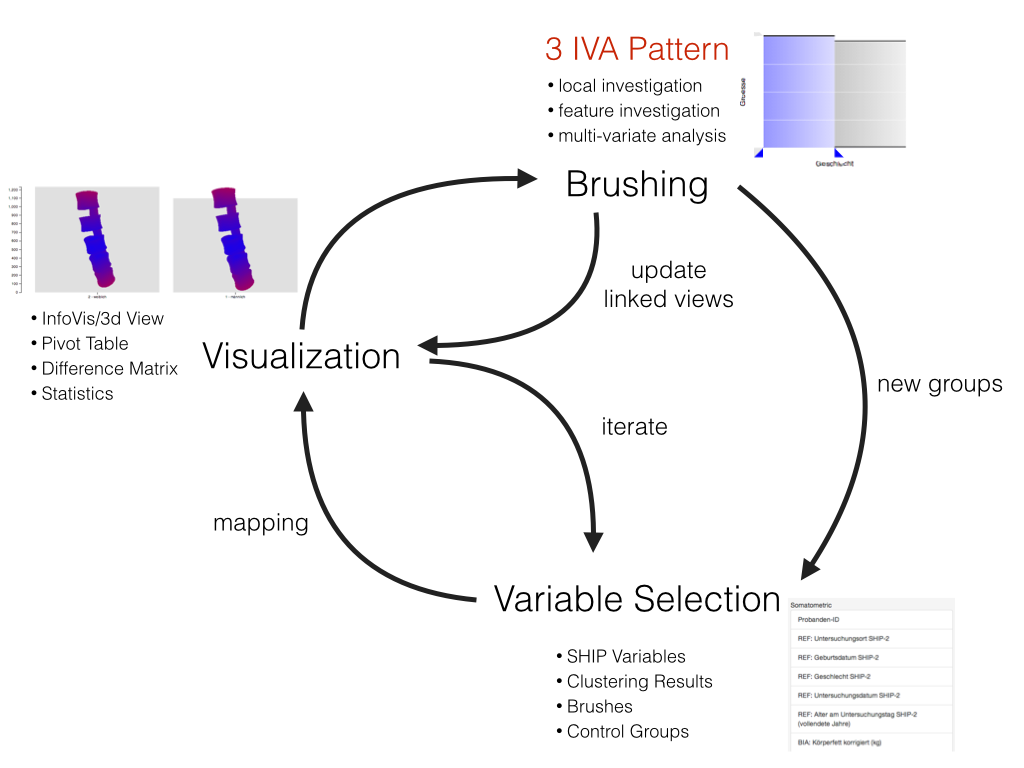
\includegraphics[width=1.5in]{figures/InteractionLoop}
%  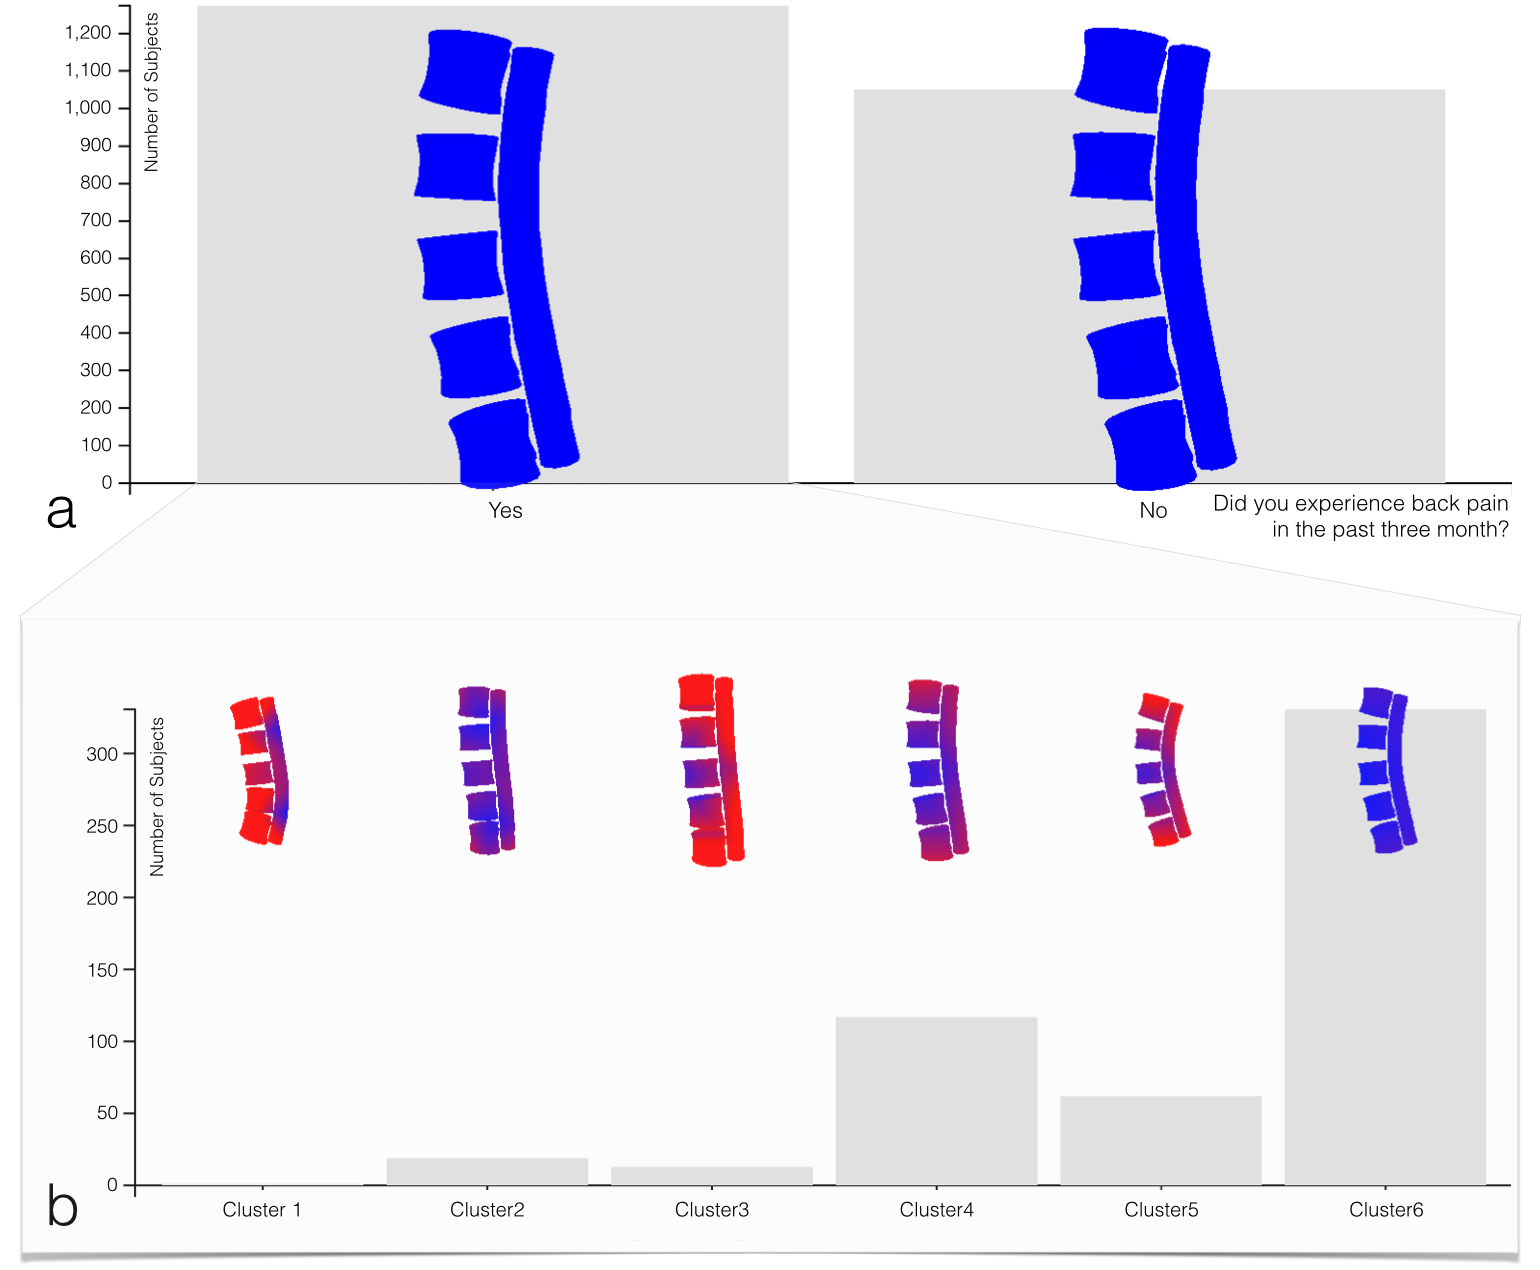
\includegraphics[width=3.5in]{figures/hypothesisbased}
%  \caption{(a) Dichotomous questionnaire answer to ``\emph{Did you experience back pain in the past three months?}''.
%  %
%  Mean shapes between the groups show no difference.
%  %
%  (b) Shape-based clustering for all subjects who suffered from back pain yields 6 groups. 
%  %
%  Note that the difference in subject count is due to the missing shape information for some subjects.
%  %
% % The total count of subjects in (b) is smaller 
%  }
%  \label{fig:hypopthesisbased}
% \end{figure}
% %
% In our use case, epidemiologists were interested in the dichotomous questionnaire answer to ``\emph{Did you experience back pain in the past three months?}''.
% %
% The mean shapes of the resulting visualization show no difference between the two groups (see Figure~\ref{fig:hypopthesisbased} (a)).
% %
% Either there are no differences or the variance information was lost in the mean shape calculation.
% %
% Since the focus is on subjects suffering from back pain, the clustering results of these subjects are then drawn into the canvas area, yielding six clusters as seen in Figure~\ref{fig:hypopthesisbased} (b).
% %
% Cluster 5 stood out for having a so-called \emph{hyperlordosis}, a strong curvature of the lumbar spine associated with back pain.
% 
% \emph{Multivariate analysis} using \emph{Cram\'{e}r's V} contingency values highlighted relationships of this cluster with joint degeneration, meat eating habits, preoccupation, back pain, neck or shoulder pain and waist circumference.
% %
% Since the prior selection only yields subjects that report back pain, the pain indicators specify the pain localization for the subjects.
% 
% It is well known that overweight is a risk factor for back pain.
% %
% While the BMI is a key figure for assessing height and weight of a subject, it does not tell anything about how the weight is distributed in the body.
% %
% Our epidemiological collaborators were interested in the correlation with waist circumference presented by this group.
% %
% Our finding follows the recent trends indicating that BMI is not a good measure for assessing the body shape, since healthy weight is dependent on many other measures \cite{Ahima2013}.
% %
% It indicates that the waist circumference rather than the BMI interacts with unusually shaped spines for subjects with lumbar back pain.
% %
% The influence of the parameter is now in the focus of further analysis.

%\com{00.46 Second: Analysis of Female subjects via clustering, selection of cluster 2, analysis using Body weight and Age. Clustering Result if 1 gives large distance between other subjects. 00.49 How are can the differences be explained?}
%\com{00.46 Feedback Body-Size/Body weight. Some features are sparse, suggestion was made to use quantile/quintile, resulting in equally occupied results. This also depends on what the user is intersted in - for clinical use the outliers may be interesting (57.30). (58.30) From perspective of a radiologists, quartile and quintiles make sense when establishing reference values for diseases; clinical relevant parameter, einflussfaktoren oder risikofaktoren zu identifizieren, je nach dem welche hypothese man verwendet.}

% ---------------------------------------------------------------------------------------------------------
\subsection{Further Feedback and Lessons Learned} \label{Lessons Learned}
%\com{ToDo: Lessons Learned der einzelnen Cases - Fokus bei Hypothesenfreier Analyse muss etwa eine gute Übersichtsvisualisierung sein, da es genau das ist was den Epidemiologen hierzu im Moment fehlt}
%
Both domain experts concluded positively over the benefits of the \emph{IVA} approach when analyzing image-based cohort study data.
%
KH emphasized the way the image data are included into information visualizations which comes much more natural to her due to her background in radiology.
%
%Both experts quickly understood the basic concepts of the visualizations and were able to 
%
Great potential is also seen in communicating insights efficiently using the presented visualizations \com{(1.08)}.
%
\paragraph{Multivariate analysis is most important for hypothesis generation.}
Both experts emphasized the potential of the \emph{multivariate analysis} capabilities of the adjacency matrix for getting insight into a large amount of features simultaneously.
%
It is also useful to verify established but still controversial risk factors, such as the metabolic syndrome for coronary heart disease and whether the data set provides even more suitable risk factors \com{(39.32)}.
%
Creating adjacency matrices for subgroups, such as different age bins can help to characterize the aging process by deriving age-specific risk factors.

\emph{Multivariate analysis} can also be improved by more ways of brushing the data as well as creating subgroups for comparison as a result of the hypothesis-driven analysis case.
%
Too small feature ranges yielding sparse groups could potentially hinder the ability to calculate statistical resilient measures, since they require a minimum amount of subjects exhibiting the selected feature ranges.
%This also has to respect the number of subjects available for epidemiological studies
%
%\paragraph{Hypothesis driven analysis would benefit from more advanced grouping.}
%While the existing brushing and linking techniques already allow the comparison of image data 
%\com{(TODO weitere Unterteilung der Variablen und anschließende Anbindung an Statistik Tools)}

\paragraph{Segmentation quality is crucial.}
The radiologist pointed out the unusual strong similarity of the L3 vertebrae throughout the population.
%
The medical explanation is that it represents an angular point of curvature of the lumbar spine.
%
A seconds explanation is the use of the L3 vertebra is initialization point of the lumbar spine model \com{(00.54)}.

The experts also emphasized that associations related to shape strongly depend on the segmentation quality.
%
The lumbar spine model used in this case study captures deformation of the spine canal well, but lacks precise definition in vertebrae height and shape.
%
Since deformation of the spine canal is the last stage of pathological lumbar spine deformation and is preceded by vertebrae deformation, the system would strongly benefit from more precise segmentation results capturing these prior changes.
%
For the visual comparison, KH proposed an abstraction of the representation into landmarks, such as centers of the vertebrae and cardinal points of the lumbar spine canal.

\paragraph{Usage of different categorizations depending on expected outcome.}
When categorizing numerical variables into equal groups it is possible to create sparse categories due to outliers, for example when analyzing body weight.
%
These outliers are only of high interest for finding pathological subjects. %but not wanted when new parameters describing risk factors are established.
%
The experts therefore suggested two modes of the tool.
%
The outlier mode still creates categories of equal size, producing sparse categories for outliers.
%
Balanced categories are created in the second mode, which uses quartiles or quintiles to set borders between categories.
\paragraph{Web technologies are well suited for rapid feedback.}
The web-based approach for both implementing the prototype as well as getting feedback via voice over ip conference calls worked very well.
%
Since the software does not need to be compiled, small changes can even be made on the fly during a testing session.
%
The large data base associated with image-based epidemiological data remains on the server machine and has not to be moved tediously using external hard disks.
%
This approach is well suited for the \emph{VDAR} approach to assess user thought processes using the think aloud technique.
%The \emph{VDAR} approach to assess user thought processes using the think aloud technique worked well with the web-based approach for both implementing the prototype as well as getting feedback via voice over ip conference calls worked very well.
%\\\\
% \rem{Although it is an entirely different approach to their usual workflows it is to highlight that the epidemiologists liked browsing through the data set in the presented manner and to dig out new information about the data.
% %
% This underlines the accessibility of \emph{IVA} tools, which amplifies the natural curiosity of the domain experts in complex medical feature associations.}

\section{Summary and Conclusion}
We presented an \emph{IVA} framework for the analysis of complex image-centric epidemiological data.
%
Hence, the framework allows for both, hypothesis-driven analysis and hypothesis generation.
%
The visualization of multivariate data using connected views and different views allows to get fast visual feedback about subject groups.
%
Brushing and linking makes the data tangible and adaptable to formulated hypotheses.
%
The use of pivot tables is familiar to epidemiologists while embracing the power of interactive adjustment of the shown features.
%
The automatic suggestion of correlations using contingency methods like \emph{Cram\'{e}r's V} triggers \emph{hypothesis generation} by highlighting features potentially overlooked by the experts.
%
Shape-based clustering assesses the variability of an anatomical structure in the context of non-image features such as disease indicators or lifestyle factors.

Epidemiologists are for the first time able to assess shape information of the lumbar spine and its influence to diseases.
%
%\com{This needs to be adjusted to fit the new Application section}
Findings from analyzing lumbar back pain using the \emph{IVA} approach range from deriving shape-based groups of subjects to detailed description of features potentially associated with the disease, such as waist circumference, alcohol consumption and attentiveness disorder.
%
%\rem{Other somatometric features, such as BMI, are not as influential as expected.}
%
\add{A number of improvements is left open for future work, such as shape brushing methods to intuitively query subjects using image data or the inclusion of more statistical methods and views that are familiar to the epidemiologists (odds ratios, box plots).}

% \begin{itemize}
% %	\item dynamic discretization of continuous variables to better fit the data distributions
% 	\item shape brushing methods to intuitively query subjects using image data,
% 	\item the inclusion of more statistical methods and views that are familiar to the epidemiologists (odds ratios, box plots), or
% 	%\item calculation of contingency differences for selected sub groups--highlighting how the feature correlation changes for a given group
% 	%\item integration of further visualization techniques, which incorporate both image and non-image data
% 	%\item support of control groups to check the resilience of observations \cite{Fletcher2012}.
% %	\item understand how the existing methods are applied to the data, iteratively adapt to the epidemiologiical workflow
% %	\item investigate which parts of the methods are applied by domain experts and what aspecunderstand how the existing methods are applied to the data, iteratively adapt to the epidemiologiical workflow
% 	\item adapt the shape visualization to explore other organ data with different variance type (such as texture of liver or white/gray matter distribution in the brain).
% \end{itemize}
% These benefits 
% - Future Work: Matrix-View of differences - more intuitive\\
% - UI more flexible by hiding UI-panes
% - More Shape-based filtering - reorder by size, curvature, etc. ...
% - Color code different Aspects - Only difference in x or y direction
% - Adjacency Matrix is symmetrical, space can be saved
% - Calculation of contingency based on the contingency differences - how does the current selection differ compared to the whole data set?
%
% To reduce the number of false positive findings, the data space can also be randomly cut in half.
% %
% Then the hypothesis then can be cross-validated for statistical soundness.
% %
% This requires a large number of subjects, especially if the investigated features are rare and only presented by a few subjects.
%
%As suggested by Fletcher and Fletcher, we plan to validate the hypothesis using the \texttt{SHIP-TREND} cohort \cite{Fletcher2012}.
% \\\\
As the number of image-centric cohort studies, participating subjects, gathered features and imaging modalities rises, and advances towards comparability between cohort studies are made, the gap between data complexity and analyzability increases.
%
Our work focuses on closing this gap, allowing the domain experts to dig deep into the data and potentially obtain unexpected findings.
%
We believe that web technologies pave the way to analyze this data in a convenient way.
%
They allow a fast exchange between users and developers and employ different devices.
%
Visual analysis shows to be a promising way to clear the view on complex epidemiological data to uncover its secrets.

%% if specified like this the section will be committed in review mode
\begin{small}
\acknowledgments{SHIP is part of the Community Medicine Research net of the University of Greifswald, Germany, which is funded by the Federal Ministry of Education and Research (grant no. 03ZIK012), the Ministry of Cultural Affairs as well as the Social Ministry of the Federal State of Mecklenburg-West Pomerania. Whole-body MR imaging was supported by a joint grant from Siemens Healthcare, Erlangen, Germany and the Federal State of Mecklenburg-Vorpommern. The University of Greifswald is a member of the ‘Centre of Knowledge Interchange’ program of the Siemens AG. This work was supported by the DFG Priority Program 1335: Scalable Visual Analytics.}
\end{small}
\clearpage
\newpage
\bibliographystyle{abbrv}
%%use following if all content of bibtex file should be shown
%\nocite{*}
\bibliography{bibliography}
\end{document}
